\chapter{Related Work}

\label{chap:related}

\section{Introduction}

Advanced Persistent Threats (APTs) represent one of the most complex challenges in the modern cybersecurity landscape. Characterized by their stealth, longevity, and multi-stage execution, APTs often evade traditional signature-based detection mechanisms. Consequently, the research community has shifted focus towards behavioral analysis and artificial intelligence (AI) to identify these sophisticated attacks. This chapter provides a detailed classification and description of existing APT detection solutions, synthesizing the state-of-the-art based on recent literature, particularly the extensive \cite{ankalaki2025cyber}. 
\section{Existing Datasets for APT Detection: A Critical Study}

If we are speaking about AI and ML, then the dataset is our number one priority --- we must carefully study all existing ones . A model is only as strong as the data it learns from, and in the highly specific domain of APT detection, this principle is even more critical. Unlike general cybersecurity datasets that capture isolated attack events, APT detection demands data that reflects multi-stage, temporally correlated, and stealthy adversarial behavior. This section is structured in three parts: (1) datasets strongly aligned with APT and CKC/MITRE ATT\&CK-based framework; (2) broader benchmark datasets from the literature that are not directly suited to APT; and (3) a review of published AI/ML works that have used these datasets, including their methods and results.

\subsection{APT-Specific Datasets With CKC/MITRE ATT\&CK Mapping}

The following datasets were selected because they carry explicit adversarial behavior annotations aligned with MITRE ATT\&CK techniques or Cyber Kill Chain phases.

\subsubsection{Linux-APT-Dataset-2024}

Karim et al. \cite{karim2024linux} published this dataset , describing it as a comprehensive APT and intrusion detection evaluation dataset for Linux systems, hosted on Mendeley Data. The dataset captures system and network logs from a Linux environment with each sample annotated against the MITRE ATT\&CK framework. Linux systems are commonly targeted by APT actors due to their prevalence in servers and critical infrastructure yet remain underrepresented in publicly available APT datasets --- a gap this dataset directly addresses. Its ATT\&CK mapping makes it directly integrable into our detection pipeline for evaluating model coverage across real adversarial techniques.

\textbf{Published ML/AI Work:} As of 2025--2026, no independent ML/AI study has yet used this dataset for model training or evaluation beyond the original description paper --- a direct consequence of the typical 6--18 month publication cycle. 

\begin{figure}[H]
    \centering
    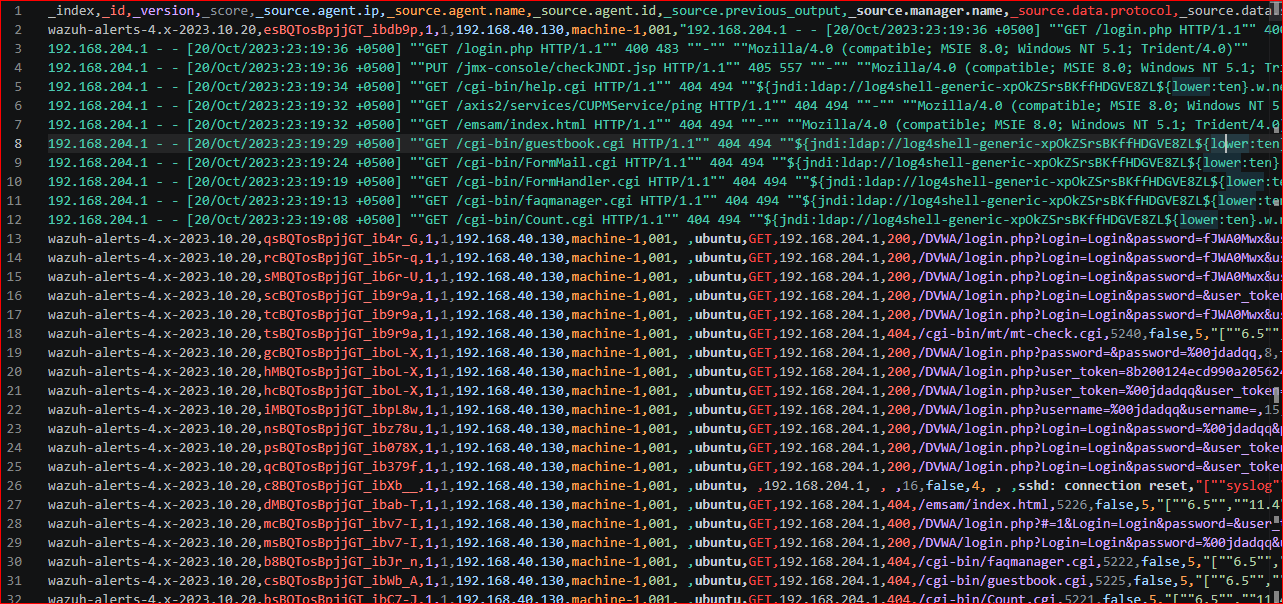
\includegraphics[width=1.0\textwidth]{figures/linux_apt.PNG}
    \caption{Visual representation of the Linux-APT-Dataset-2024}
    \label{fig:linux_apt_data}
\end{figure}


\subsubsection{LOTL APT Red Team Dataset}

Hosted on Kaggle (cyberprince/lotl-apt-red-team-dataset), this dataset focuses on \textbf{Living-off-the-Land (LOTL)} APT techniques --- adversaries using legitimate system tools (PowerShell, WMI, certutil) instead of custom malware. LOTL attacks are among the most challenging to detect because they produce minimal distinctive signatures and blend seamlessly with normal administrative activity. This dataset is essential for evaluating the model's ability to detect technique-level anomalies rather than simple malware signatures.

\subsubsection{Windows APT Persistence Techniques Dataset (2025)}

Riahi and Debatty \cite{rahal2025windows} published this dataset at IEEE ICIN 2025, described as \textit{"Dataset of APT Persistence Techniques on Windows Platforms Mapped to the MITRE ATT\&CK Framework"}, available on Mendeley Data. It provides comprehensive persistence behavior traces mapped to ATT\&CK TA0003 (Persistence), with a focus on tactics employed by Chinese threat actors. The \textbf{Persistence} tactic is one of the defining characteristics of APTs --- adversaries maintain long-term, undetected foothold within compromised systems --- making this dataset directly relevant to the Installation and C2 phases of the CKC.

\textbf{Published ML/AI Work:} This dataset \cite{rahal2025windows} was published at an IEEE conference in early 2025 and currently has only 2 Scopus citations; no ML/AI study has yet used it independently.  Ling et al. (2023) further surveyed adversarial attacks against Windows PE malware detection, demonstrating the critical importance of Windows-specific attack vectors and the robustness challenges any model must address on this platform [4].

\subsubsection{KAPT-2024}

 \cite{ambalangodage2024kapt} introduced KAPT-2024 in \textit{"A Relevant Feature Identification Approach to Detect APTs in HTTPS Traffic"} , generated using the KExtractor tool and hosted on GitHub. The dataset focuses on HTTPS-encrypted traffic --- a realistic and challenging scenario since APT actors increasingly use encrypted channels to blend C2 communication into legitimate traffic. The paper itself constitutes the primary reference for this dataset and presents a feature identification approach as part of the same publication; no independent research team has yet exploited it.

\textbf{Published ML/AI Work:} The original paper by \cite{ambalangodage2024kapt} presents a relevant feature identification pipeline applied to KAPT-2024 as illustrated in Figuer \ref{fig:kapt_data}.  

\begin{figure}[H]
    \centering
    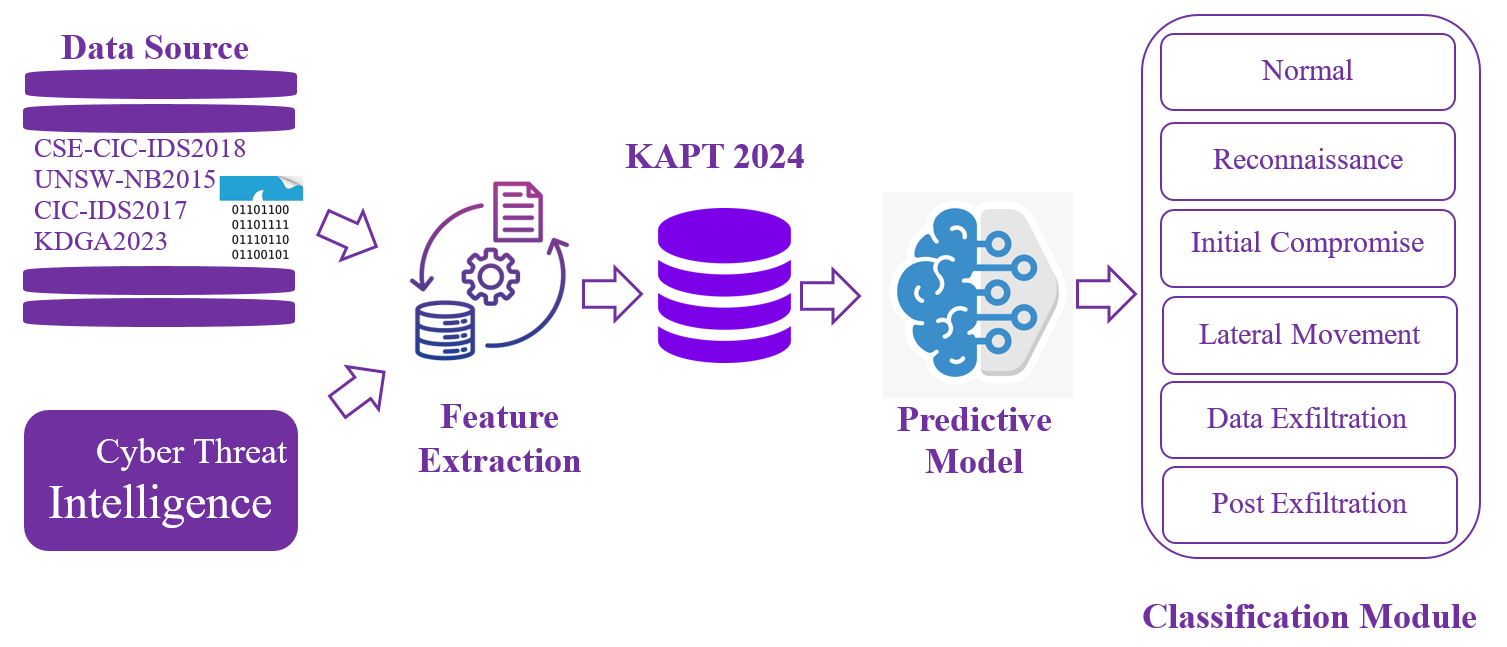
\includegraphics[width=0.7\textwidth]{figures/kapt.png}
    \caption{Visual overview of the KAPT-2024 dataset}
    \label{fig:kapt_data}
\end{figure}

\subsubsection{CloudAPT Dataset}

Published via the National Research Council of Canada's digital repository, this dataset covers APT attack steps in cloud environments. Cloud-specific APT datasets are currently underrepresented in the community, making this resource particularly valuable as enterprise infrastructure continues its shift to cloud platforms.

\subsubsection{MLAPT Dataset}

The MLAPT dataset accompanies the paper \textit{"A Cyber Kill Chain Approach for Detecting Advanced Persistent Threats"} (Ancona et al.), available both at the GitHub repository \footnote{GitHub: \url{https://github.com/alessandro-ancona/APT_detector/blob/master/MLAPT_dataset.csv}} and via the Loughborough University repository. This dataset is particularly aligned with our work because it is explicitly structured around the \textbf{Cyber Kill Chain model} --- the primary threat modeling framework of this thesis. Alerts are labeled according to CKC phases, making it a natural benchmark for evaluating stage-aware APT detection models and a direct validation ground for our proposed sequential detection architecture.

\subsubsection{ATLAS audit logs}

sourced from \cite{alsaheel2021atlas} — ATLAS audit logs, available on GitHub. The dataset simulates a 10-day enterprise environment in an isolated network, with both single-host (S-1 to S-4) and multi-host lateral movement attacks (M-1 to M-6). On average, each attack scenario produces 19,750 entities and around 284,000 events per attack. Benign behavior is realistically simulated alongside attacks — users browse websites, download files, and interact with remote servers within an 8-hour working-day window.

\subsubsection{CICAPT-IIoT}

Ghiasvand et al. \cite{ghiasvand2024cicapt} introduced CICAPT-IIoT in arXiv preprint 2407.15130 (2024), described as \textit{"CICAPT-IIoT: A Provenance-Based APT Attack Dataset for IIoT Environment"}, available via CIC Research Canada and Kaggle. The dataset covers more than 4 GB of IIoT network traffic records integrating 20 MITRE ATT\&CK techniques like it shows in the figuer \ref{fig:cicapt_iot_data}. Its \textbf{provenance-based} approach records the causal chain of system events (file reads, process forks, network connections) rather than only network flows .

\textbf{Published ML/AI Work Using CICAPT-IIoT \cite{ghiasvand2024cicapt}:} One important study has directly applied a CNN2D-based deep learning model to this dataset.

\begin{figure}[H]
    \centering
    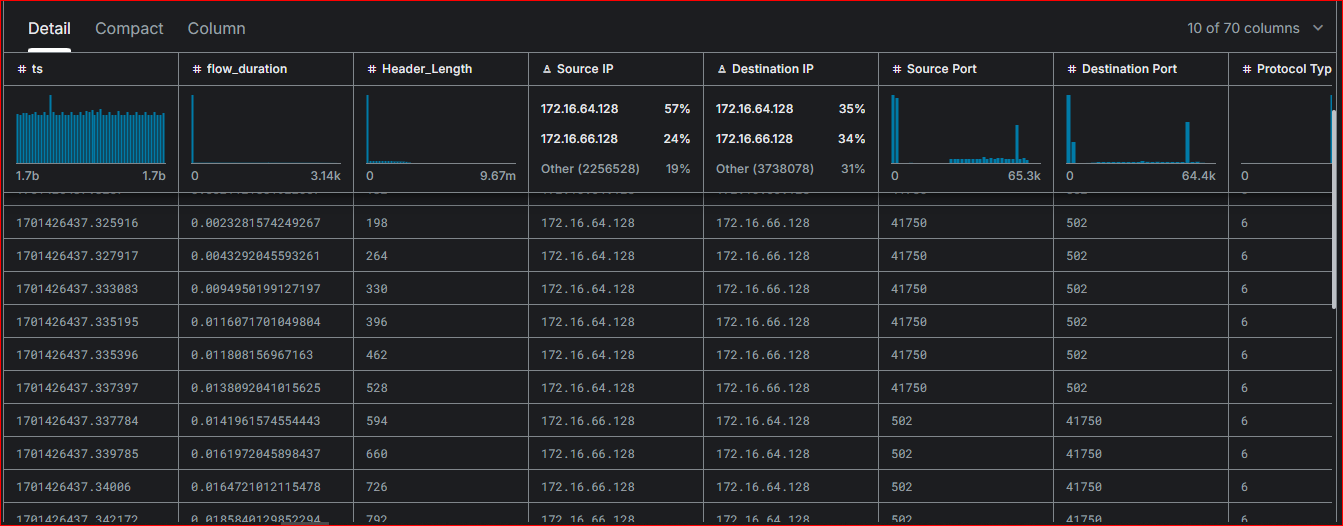
\includegraphics[width=1.0\textwidth]{figures/iot.PNG}
    \caption{Visual overview of the CICAPT-IIoT dataset}
    \label{fig:cicapt_iot_data}
\end{figure}

\begin{table}[H]
\centering

\caption{Summary Table --- Datasets With CKC/MITRE ATT\&CK Mapping}
\smallskip
\label{tab:summry_dataset}

\begin{tabular}{|p{0.3\linewidth}|p{0.2\linewidth}|p{0.2\linewidth}|p{0.3\linewidth}|}
\hline
\textbf{Dataset} & \textbf{Mapping} & \textbf{Environment} & \textbf{Key Relevance to Our Work} \\
\hline
Linux-APT-Dataset-2024 \cite{karim2024linux} & MITRE ATT\&CK & Linux & Linux-specific labeled APT logs \\
\hline
MLAPT & CKC Phases & Network & CKC-aligned alert labeling \\
\hline
KAPT-2024 \cite{ambalangodage2024kapt} & MITRE ATT\&CK & HTTPS Traffic & Encrypted C2 detection \\
\hline
Windows APT Persistence 2025 \cite{rahal2025windows} & MITRE ATT\&CK & Windows & Persistence tactic (TA0003) \\
\hline
CICAPT-IIoT \cite{ghiasvand2024cicapt} & MITRE ATT\&CK & IIoT & Provenance graphs, CNN2D validated \\
\hline
TRAM/TTP Mapping & MITRE ATT\&CK & CTI Text & NLP/LLM TTP extraction \\
\hline
APT Audit Logs (5 Groups) & MITRE ATT\&CK & Multi-env & Multi-group generalization \\
\hline
LOTL APT Red Team & MITRE ATT\&CK & Windows & Living-off-the-land detection \\
\hline
CloudAPT & Likely ATT\&CK & Cloud & Cloud-based APT scenarios \\
\hline
LMD Collections \cite{mabrouk2025lmdg} & Partial ATT\&CK & Network & Lateral movement evaluation \\
\hline
\end{tabular}
\end{table}

\subsection{APT-Specific Datasets Without Explicit Mapping}

\begin{itemize}
    \item \textbf{DAPT 2020} \cite{myneni2020dapt}: Purpose-built for APT detection (\textit{"DAPT 2020 - Constructing a Benchmark Dataset for Advanced Persistent Threats"}, Kaggle). Its annotation scheme does not follow the MITRE ATT\&CK taxonomy, limiting ATT\&CK-coverage evaluation.
    \item \textbf{Unraveled APT Dataset} \cite{myneni2023unraveled}: A semi-synthetic dataset for APT research (Kaggle). Semi-synthetic nature means some behaviors may not faithfully represent real-world APT tradecraft.
    \item \textbf{LANL Multi-Source Cybersecurity Events}: Real-world dataset from Los Alamos National Laboratory containing 90 days of anonymized internal network events (authentication logs, process events, DNS queries). Highly realistic and temporally rich, associated with an RNN attention mechanism paper (arXiv:1803.04967), but lacks APT-specific labels and CKC annotations.
    \item \textbf{CIC-IDS2018} \cite{hewapathirana2025comparative}: Available on Kaggle and AWS; used in APT-adjacent studies but focused on individual attack types rather than multi-stage campaigns.
\end{itemize}


\subsection{Broader Cybersecurity Datasets --- Not Directly Suited for APT}

The survey by \cite{ankalaki2025cyber}. covers an extensive catalog of cybersecurity benchmark datasets across seven categories. While these datasets are widely adopted for evaluating ML/DL models in general intrusion detection, they are \textbf{not directly suited to our APT multi-stage detection objective} for two primary reasons: (1) they lack MITRE ATT\&CK or CKC annotations that would allow stage-aware evaluation, and (2) most capture isolated, single-stage attack events rather than the temporally correlated, multi-phase sequences that define APT campaigns. They nonetheless form the foundational literature landscape from which our work departs.

\subsubsection{Network Traffic-Based Datasets}

As documented in \cite{ankalaki2025cyber}, this is the most studied category in intrusion detection research:

\begin{itemize}
    \item \textbf{KDD Cup 1999 / NSL-KDD}: Historically the most cited IDS datasets, containing four attack categories (DoS, U2R, R2L, Probe). Widely criticized for outdated traffic patterns, redundant data, and unrealistic scenarios that do not reflect modern APT techniques \cite{ankalaki2025cyber}.
    \item \textbf{UNSW-NB15 (2015)}: Ten attack categories including backdoors and shellcode, generated over 31 hours of emulated traffic. More diverse than KDD, but attacks remain isolated events rather than multi-stage campaigns \cite{ankalaki2025cyber}.
    \item \textbf{CICIDS2017}: One of the most comprehensive modern IDS datasets --- 3.1M flows, 8 attack types (SQL injection, DoS, DDoS, botnet, brute force, etc.) over 5 days. Despite its richness, it lacks APT-specific attack chains or CKC/ATT\&CK annotations \cite{ankalaki2025cyber}.
    \item \textbf{LITNET 2020}: Recent dataset with 12 attack types from real network traffic, small in size and focused on known cataloged signatures \cite{ankalaki2025cyber}.
    \item \textbf{HIKARI-2021}: Covers bruteforce variants and cryptomining over 39 hours of real traffic \cite{ankalaki2025cyber}.
\end{itemize}

The fundamental limitation of this entire category for our purposes is that they capture \textit{what happened} (attack type), not \textit{where in the attack lifecycle it happened} (kill chain phase).

\subsubsection{Malware and Android-Based Datasets}

\begin{itemize}
    \item \textbf{CIC-AndMal2017 / CCCS-CIC-AndMal-2020}: Android malware datasets covering spyware, trojans, adware, ransomware. Useful for endpoint-level malware classification (CKC Phase 2 --- Weaponization) but provide no multi-stage campaign context.
    \item \textbf{SoReL-20M}: Over 20 million malware samples. Impressive scale for malware classification but no temporal or campaign-level APT structure.
\end{itemize}

\subsubsection{IoT Traffic-Based Datasets}

\begin{itemize}
    \item \textbf{TON-IoT (2020)}: Nine attack types in IoT environments, simulated traffic. LSTM achieved 97\% accuracy and CNN 99\% \cite{ankalaki2025cyber}. However, attacks are individually labeled without CKC phase structure.
    \item \textbf{Bot-IoT (2019)}: 46-feature botnet detection dataset where LSTM achieved $\sim$98\% and SVM $\sim$99\% \cite{ankalaki2025cyber}. No CKC/ATT\&CK phase annotations.
    \item \textbf{X-IIoTID (2021)}: 18 attack types including reconnaissance, lateral movement, and C2 --- features partially overlapping with CKC phases. GRU achieved 99.46\% accuracy \cite{ankalaki2025cyber}. Its lack of explicit CKC mapping limits its use for stage-aware evaluation, though it is the closest in this category to APT-relevant data.
\end{itemize}

Many research works and articles use this type of dataset and present their solutions as "APT detection" frameworks. However, in reality they are not, due to the lack of true APT characteristics in these datasets --- specifically, the long-term temporal sequencing of attacks and the correlation between these multi-stage sequences.

\subsubsection{Limitations of APT Stage-Aware Detection}

The review of datasets in \cite{ankalaki2025cyber} reveals several  limitations when applied to the APT detection problem:

\begin{enumerate}
    \item \textbf{Narrow Attack Scope}: Datasets like MQTT-IoT-IDS2020 provide few attack classes, restricting model generalizability to the wide variety of real-world APT techniques.
    \item \textbf{Outdated or Simulated Traffic}: Older datasets (Bot-IoT 2019) do not capture modern APT techniques; simulation-based datasets (TON-IoT) fail to reproduce the complexity of real-world APT campaigns.
    \item \textbf{Absence of Stage Annotations}: The most critical limitation --- none of the general benchmark datasets in \cite{ankalaki2025cyber} provide kill-chain phase or ATT\&CK technique annotations, making them unsuitable for evaluating the stage-aware component of our framework.
    \item \textbf{Class Imbalance}: APT-related traffic constitutes a minuscule fraction of total network activity, as confirmed by CICAPT-IIoT's $\sim$95\%/5\% normal-to-attack ratio.
    \item \textbf{Lack of Provenance Context}: Standard flow-based datasets discard causal relationships between events (which process spawned which network connection), essential for graph-based APT detection.
\end{enumerate}


\section{Classification of Solutions}
\label{sec:classification}

Based on the comprehensive analysis provided by \cite{ankalaki2025cyber}, detection solutions for cyber-attacks and APTs can be broadly categorized based on the underlying algorithmic evolution and learning paradigms. The classification progresses from traditional statistical methods to advanced generative models.

\subsection{Traditional Machine Learning (ML) Approaches}
Traditional ML approaches constitute the foundational layer of intelligent detection. As highlighted in \cite{ankalaki2025cyber}, these are further divided based on the availability of labeled data:
\begin{itemize}
    \item \textbf{Supervised Learning:} These algorithms require fully labeled datasets (benign vs. malicious). They are widely used for malware classification and detecting known intrusion patterns but struggle with zero-day attacks.
    \item \textbf{Unsupervised Learning:} These methods operate on unlabeled data, aiming to discover hidden structures or anomalies. In the context of APTs, unsupervised learning is critical for identifying deviations from "normal" network baselines without prior knowledge of the attack signature.
    \item \textbf{Semi-supervised Learning:} A hybrid approach that utilizes a small amount of labeled data alongside a large volume of unlabeled data, addressing the scarcity of annotated APT datasets.
\end{itemize}

\subsection{Deep Learning (DL) Approaches}
Deep Learning represents a subset of ML that utilizes multi-layered neural networks to learn hierarchical representations of data. \cite{ankalaki2025cyber} emphasize that DL models outperform traditional ML in handling unstructured high-dimensional data, such as raw network traffic bytes or system log sequences. Key architectures in this category include Convolutional Neural Networks (CNNs) and Recurrent Neural Networks (RNNs).

\subsection{Generative Artificial Intelligence (GenAI) Approaches}
The most recent evolution in detection strategies involves Generative AI. Unlike discriminative models that separate classes, generative models (such as VAEs and GANs) learn the underlying distribution of the data to generate new instances. According to \cite{ankalaki2025cyber}, GenAI is revolutionizing cybersecurity by enabling:
\begin{enumerate}
    \item \textbf{Advanced Anomaly Detection:} By learning the exact distribution of benign traffic, any deviation-even subtle-can be flagged with high precision.
    \item \textbf{Data Augmentation:} Generating synthetic attack data to train models, addressing the critical lack of real-world APT samples.
    \item \textbf{Adversarial Defense:} Simulating attacks to harden defense systems.
\end{enumerate}




\section{Description of Solutions: Review of AI/ML on APT Datasets}
\label{sec:description}

This section details the technical mechanisms of the algorithms identified in the classification, evaluating their specific application to APT detection as discussed in \cite{ankalaki2025cyber}.

\subsection{Machine Learning Solutions}

\subsubsection{Support Vector Machines (SVM)}
SVM is a supervised learning algorithm that constructs a hyperplane or set of hyperplanes in a high-dimensional space to separate classes (e.g., Normal vs. Attack). 
\begin{equation}
    f(x) = \text{sign}(\sum_{i=1}^{n} \alpha_i y_i K(x_i, x) + b)
\end{equation}
As noted in \cite{ankalaki2025cyber}, SVMs are effective for high-dimensional data but entail high computational costs during the training phase, making them less suitable for real-time processing of massive network flows.

\subsubsection{Random Forest (RF) and Decision Trees}
Decision Trees (DT) provide high interpretability by splitting data based on feature values. Random Forest (RF) improves upon DT by aggregating multiple trees (bagging) to reduce overfitting. \cite{ankalaki2025cyber} report that RF achieves high accuracy (often exceeding 99\%) in detecting specific attack types like DDoS and Botnets within IoT environments, making it a robust baseline for APT stage detection.

\subsubsection{Naive Bayes (NB)}
Based on Bayes' theorem (as shown in Equation~\ref{eq:bayes}) with an assumption of feature independence, NB is computationally efficient. While it lacks the nuance to detect complex, correlated APT behaviors, it serves as a fast filter for initial traffic classification \cite{ankalaki2025cyber}.

\begin{equation}
    P(A|B) = \frac{P(B|A) P(A)}{P(B)}
    \label{eq:bayes}
\end{equation}

\paragraph{Case Study 1: Real-Time Early Multi-Stage Attack Detection \protect\cite{takey2021real}}
\cite{takey2021real} proposed a novel real-time framework combining Machine Learning and the MITRE ATT\&CK framework for early multi-stage attack detection through static analysis of Windows Portable Executable (PE) binaries.

\textbf{Architecture Used:} The system is composed of three major interconnected components:
\begin{itemize}
    \item \textbf{Run-Time Engine:} The core component, built on Microsoft Sysmon, monitors two critical OS events --- Event ID 1 (Process Creation) and Event ID 15 (FileCreateStreamHash for browser downloads). Upon detection, it forwards the executable to the next stage for analysis.
    \item \textbf{Feature Extractor:} Parses the static PE binary using Python's pefile library and extracts 259 features derived from three MITRE data sources: API calls (F1--F244), Binary File Metadata (Export/Import Table, Architecture, IsPacked, IsDebug, ValidHeader, etc.), and DLL Monitoring (DLL count).
    \item \textbf{ML Engine + MITRE Adversary Technique Module:} Receives the extracted features, classifies the binary as malign or benign, and --- if malicious --- maps it to the corresponding MITRE ATT\&CK adversary techniques (Execution, Persistence, Privilege Escalation, Defense Evasion, Credential Access, Discovery, Lateral Movement, Collection, Impact) to predict the stages the malware will execute during the attack.
\end{itemize}

\textbf{Methodology \& Dataset:} The dataset was built by collecting malware samples from publicly available repositories, Cert-In India, and honeypots (labeled as malign), and by extracting all executables from a freshly installed Windows 10 system (labeled as benign). The labeled dataset contains 7,699 entries (4,076 malign, 3,623 benign). A total of 259 features were identified based on MITRE TTP analysis and literature review. Principal Component Analysis (PCA) was applied to reduce the feature space from 257 to 160 features. Five classical ML models were trained and evaluated: Naive Bayes, Decision Tree, KNN, SVM, and Random Forest.

\textbf{Results \cite{takey2021real}:} The proposed system was tested on 6,000 unpacked malware samples and achieved an overall accuracy of 98.18\% after PCA-based feature reduction. The system successfully predicted the adversary techniques executed by the malware and mapped binaries to their corresponding MITRE ATT\&CK phases in real time. The major additional contribution of this work is the identification of over 240 Windows API calls mapped to 300+ MITRE TTPs, enabling fine-grained multi-stage attack stage prediction.

\begin{figure}[H]
    \centering
    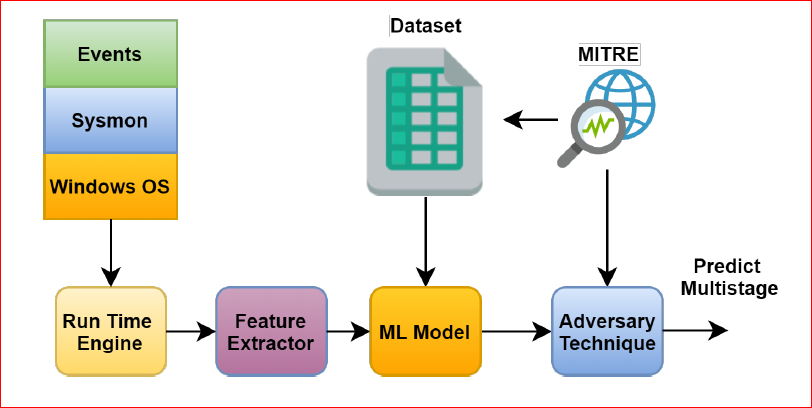
\includegraphics[width=0.7\linewidth, trim=3pt 4pt 4pt 4pt, clip]{figures/archi.PNG}
    \caption{Overall Architecture of Real-Time Early Multi-Stage Attack Detection \protect\cite{takey2021real}}
    \label{fig:architecture}
\end{figure}

\paragraph{}
Daoud and Hamdi proposed DTB-IDS, a decision-tree-based intrusion detection system for multi-level APT detection using MITRE ATT\&CK mapping. The model was trained on a merged dataset of UWF-ZeekData24 and NF-UQ-NIDS-v2, containing 628{,}415 flow records, and achieved 99.2\% binary accuracy, 99.1\% tactic F1, and 99.4\% technique micro-F1. The authors also reported strong cross-dataset validation on CICIDS2017, confirming the robustness and interpretability of the approach \cite{daoud2026dtbids}.


\subsubsection{Deep Q-Network (DQN)}
DQN combines Q-learning \cite{watkins1989learning,watkins1992qlearning} with deep neural networks to approximate the action-value function \( Q(s,a;\theta) \approx Q^*(s,a) \), replacing the infeasible lookup table of classical Q-learning. The agent follows an $\epsilon$-greedy policy and trains by minimizing the TD loss:

\[ 
L(\theta) = \mathbb{E} \left[ \left( r + \gamma \max_{a'} Q(s',a';\theta^-) - Q(s,a;\theta) \right)^2 \right] 
\]

Two key mechanisms stabilize training: a target network $\theta^-$ (frozen periodically) for stable TD targets, and experience replay (random mini-batch sampling from a replay buffer) to break temporal correlations \cite{mnih2015human}.


\paragraph{Case Study--- OGE-DQN: Deep Q-Network for Intrusion Detection}
Saad, A.M.S.E. \& Yildiz, B. (2023) --- ``Reinforcement Learning for Intrusion Detection'' \cite{saad2023reinforcement}.

\textbf{Approach} \\
The authors construct a custom OpenAI Gym environment that wraps the NSL-KDD dataset and serves network traffic records to the agent as sequential observations. The environment follows a standard RL loop: at each step, the agent receives a state $S_t$ (a 41-dimensional feature vector of one traffic record), selects an action $A_t \in \{0 \text{ (Normal)}, 1 \text{ (Intrusion)}\}$, and receives a reward $R_{t+1}$ according to a simple correctness-based reward function:
\[
R = \begin{cases} 
+1 & \text{if action matches the ground-truth label} \\ 
-1 & \text{otherwise} 
\end{cases}
\]

The agent is a Deep Q-Network (DQN) \cite{mnih2015human}, which uses a feed-forward neural network with two hidden layers (50 neurons $\rightarrow$ 10 neurons) to approximate the Q-value function. The network is optimized via the Bellman update using two key stability techniques:
\begin{itemize}
    \item \textbf{Experience Replay:} Transitions $(S_t, A_t, R_{t+1}, S_{t+1})$ are stored in a replay buffer and randomly sampled in mini-batches to break temporal correlations.
    \item \textbf{Target Network:} A separate, slowly updated copy of the main network is used to compute target Q-values, preventing oscillating updates.
\end{itemize}

Training uses an $\epsilon$-greedy exploration strategy with $\epsilon$ decaying over time from 1.0 toward a minimum --- allowing the agent to shift from random exploration to exploitation of learned patterns. The optimal configuration was found at 800 training iterations, 100 steps per episode, batch size of 64, using the full dataset.

\textbf{Published Results}
\begin{table}[H]
\centering
\caption{Performance comparison of OGE-DQN and literature models on NSL-KDD dataset.}
\medskip
\resizebox{1.0\textwidth}{!}{%
\begin{tabular}{|l|c|c|c|c|}
\hline
\textbf{Experiment} & \textbf{Accuracy} & \textbf{Precision} & \textbf{Recall} & \textbf{F1-Score} \\ \hline
RL Experiment 1 (50\% data, 400 iter.) & 86.80\% & 82.45\% & 86.55\% & 84.45\% \\ \hline
RL Experiment 2 (100\% data, 800 iter.) & 93.12\% & 96.83\% & 95.90\% & 96.36\% \\ \hline
DQN --- Lopez-Martin et al. \cite{lopez2020application} & 87.87\% & 89.33\% & 89.37\% & 89.35\% \\ \hline
DDQN --- Ma \& Shi \cite{ma2020idsgan} & 82.09\% & 84.11\% & 82.09\% & 82.43\% \\ \hline
\end{tabular}%
}
\end{table}

\begin{figure}[H]
    \centering
    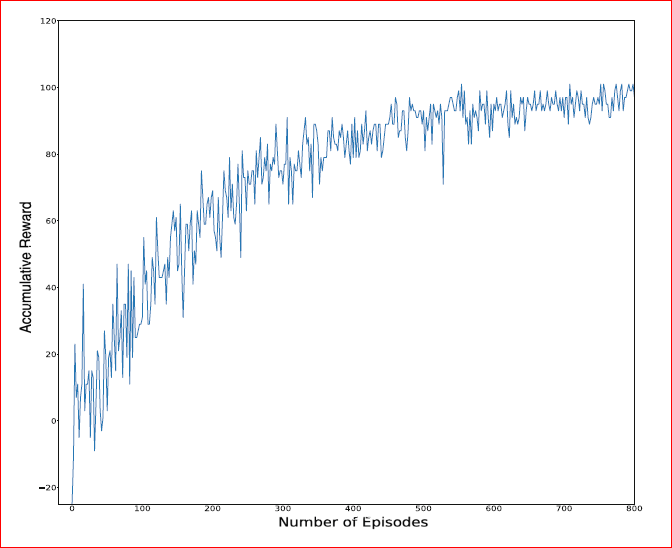
\includegraphics[width=0.7\linewidth, trim=3pt 4pt 4pt 4pt, clip]{figures/rl_resu.PNG}
    \caption{RL Agent Learning Curve (accumulative reward over episodes)}
    \label{fig:RL}
\end{figure}

The best experiment (Experiment 2) outperforms all comparable DRL methods in the literature on the same dataset. The key contribution is the standardized OpenAI Gym IDS environment, which for the first time allows other researchers to benchmark DRL agents against a reproducible, interoperable IDS testbed \cite{saad2023reinforcement}.





\subsection{Deep Learning Solutions}

\subsubsection{Convolutional Neural Networks (CNN)}
Originally designed for image processing, CNNs are applied to cybersecurity by treating network traffic as images or matrices. They excel at extracting spatial features (local patterns) from traffic payloads. \cite{ankalaki2025cyber} highlights their utility in malware classification where binary executables are visualized as grayscale images.

\textbf{Case Study: CNN2D-based framework \cite{SharmilaD2026CNN2D}}

One important study \cite{SharmilaD2026CNN2D} has directly applied a deep learning model to this dataset. The paper proposes a \textbf{CNN2D-based framework} for IoT cyberattack detection on CICAPT-IIoT, following an 8-step pipeline:

1. Data acquisition from the CICAPT-IIoT dataset (attack records + balanced normal subset)
2. Preprocessing: null value handling, Label Encoding, shuffling, normalization
3. Advanced feature engineering: correlation analysis, PCA for dimensionality reduction, temporal windowing
4. Feature scaling: both Min-Max and Z-score normalization tested
5. \textbf{2D reshaping} of feature vectors into matrix format (image-like) to enable CNN2D spatial processing
6. Train/test split
7. Real-time prediction deployment

The CNN2D architecture uses 3 convolutional layers (3$\times$3 and 5$\times$5 kernels), ReLU activation, Max-Pooling, Dropout (rate = 0.3), and Softmax output. Hyperparameters were tuned via grid search + cross-validation (batch size: 128, learning rate: 0.001, optimizer: Adam, loss: categorical cross-entropy).


\begin{table}[H]
\centering
\caption{CNN2D vs. Baseline Models on CICAPT-IIoT \protect\cite{ghiasvand2024cicapt}}
\medskip
\begin{tabular}{|p{0.3\linewidth}|p{0.15\linewidth}|p{0.15\linewidth}|p{0.15\linewidth}|p{0.15\linewidth}|}
\hline
\textbf{Algorithm} & \textbf{Accuracy (\%)} & \textbf{Precision (\%)} & \textbf{Recall (\%)} & \textbf{F1-Score (\%)} \\
\hline
\textbf{CNN2D (Proposed)} & \textbf{99.78} & \textbf{99.7} & \textbf{99.8} & \textbf{99.75} \\
\hline
Logistic Regression & 99.70 & 99.0 & 99.8 & 99.70 \\
\hline
Random Forest & 96.00 & 95.2 & 96.5 & 95.80 \\
\hline
SVM & 94.00 & 93.4 & 94.1 & 93.70 \\
\hline
\end{tabular}
\end{table}

For scalability, the CNN2D model maintained \textbf{99.78\% accuracy on 50,000 records} (avg. prediction time: 1.2 s) and \textbf{99.65\% accuracy on 200,000 records} (avg. prediction time: 3.8 s), confirming strong discriminative capacity even on the highly imbalanced dataset ($\sim$95\% normal / $\sim$5\% attack). This result directly validates CICAPT-IIoT \cite{ghiasvand2024cicapt} as a viable training and evaluation benchmark and provides a strong performance reference point for our own experimental phase.

\subsubsection{Recurrent Neural Networks (RNN) and LSTM}
Given that APTs are temporal, multi-stage attacks, standard feed-forward networks often fail to capture the sequence of events. RNNs address this by maintaining a "memory" of previous inputs. Specifically, Long Short-Term Memory (LSTM) networks are crucial for APT detection because they solve the vanishing gradient problem, allowing the model to learn long-term dependencies.
\begin{equation}
    f_t = \sigma(W_f \cdot [h_{t-1}, x_t] + b_f)
\end{equation}
This capability allows LSTMs to correlate a "Reconnaissance" event (Stage 1) with an "Exfiltration" event (Stage 7) that occurs days or weeks later \cite{ankalaki2025cyber}.

\textbf{Case Study: AISL \cite{yue2024aisl}}

\textbf{Approach}
AISL operates in three main stages:

\textbf{Stage 1 --- Provenance Graph Construction:} Heterogeneous audit data (system calls, DNS logs, network traffic) is unified through a custom Network Event Ontology with 5 core concepts (host, subject, object, event, tag) and 10 relationships. This solves the semantic gap between Windows and Linux audit formats.

\textbf{Stage 2 --- Attack Intent Tagging:} Two tag types are assigned --- trustworthiness tags (BA = Benign Authentic, BE = Benign, UN = Unknown) and confidentiality tags (SC = Secret, PR = Private, PU = Public). Tags propagate through the graph using rule-based policies, identifying potential attack behaviors to increase positive samples --- a key innovation solving the APT data imbalance problem.

\textbf{Stage 3 --- LSTM Sequence Model:} Attack and non-attack sequences are extracted from the provenance graph, converted to lemmatized abstract text, and fed into an LSTM classifier with Conv1D, dropout, and dense layers. Oversampling (mutation-based) and undersampling (similarity-based) balance the training set before model training.

\textbf{Published Results}
\begin{table}[H]
\centering
\caption{AISL Detection Results at Entity and Event Levels}
\begin{tabular}{|l|c|c|c|c|}
\hline
\textbf{Method} & \textbf{Entity Precision} & \textbf{Entity Recall} & \textbf{Entity F1} & \textbf{Event F1} \\
\hline
Graph-traversal & 20.36\% & 100.00\% & 33.83\% & 38.51\% \\
Non-optimized & 74.08\% & 53.12\% & 61.87\% & 65.21\% \\
SVM & 80.32\% & 88.06\% & 84.01\% & 89.56\% \\
ATLAS & 91.06\% & 97.29\% & 93.76\% & 99.88\% \\
\textbf{AISL (Proposed)} & \textbf{93.05\%} & \textbf{98.12\%} & \textbf{95.36\%} & \textbf{99.91\%} \\
\hline
\end{tabular}
\end{table}

Accuracy per attack scenario reaches 99.96--100\% at the event level, with an average entity-level accuracy of 99.98\% across all 10 APT attacks.

\subsubsection{Graph Neural Networks (GNN)}


Graph Neural Networks (GNNs) are deep learning models designed to operate on
graph-structured data, where information is represented as \textbf{nodes}
(entities) and \textbf{edges} (relationships). They learn node representations
by aggregating and transforming feature information from neighboring nodes
across multiple layers.

\subsubsection{Key Types}

\begin{itemize}
    \item \textbf{GCN (Graph Convolutional Network):} Aggregates neighbor
    features using fixed, structure-based weights derived from the normalized
    adjacency matrix. It is simple and computationally efficient, but treats
    all neighbors equally.

    \item \textbf{GAT (Graph Attention Network):} Extends GCN by introducing
    a self-attention mechanism that learns to assign different importance
    weights to different neighbors during aggregation. Multi-head attention
    is used to stabilize and enrich the learning process.

    \item \textbf{GraphSAGE:} Samples a fixed-size neighborhood for each node
    rather than using the full graph, making it highly scalable to large
    graph datasets.

    \item \textbf{GGNN (Gated Graph Neural Network):} Incorporates Gated
    Recurrent Units (GRUs) into the propagation step to capture long-range
    dependencies between nodes.
\end{itemize}

Think of a network as a city map --- computers are buildings, connections are roads. An APT attacker does not strike once; they hop quietly from building to building toward their target. A GNN models this entire map at once, detecting suspicious \textit{patterns of movement} rather than isolated events --- making it the natural fit for APT detection.

The key distinction is that \textbf{GAT learns \textit{who} to pay attention
to}, while GCN treats all neighbors equally --- making GAT especially suitable
for tasks such as APT detection, where certain graph connections carry
significantly higher suspicion than others.

This sections adopts the classification by Zhong et al. (2024) \cite{zhong2024}, organizing GNN-based IDS along three axes:
\begin{itemize}
    \item \textbf{Graph Construction (Data $\rightarrow$ Graph):} Static graphs (original, enriched, transformed, heterogeneous) or Dynamic graphs (snapshots, sketching).
    \item \textbf{Network Design (Graph $\rightarrow$ Feature):} Network-based IDS (NIDS) at node/edge/graph-level, or Host-based IDS (HIDS) via provenance/system call graphs.
    \item \textbf{Model Deployment:} Strategy (centralized, federated, parallel) and Domain (IoT, CPS, etc.). Figure \ref{fig:gnn1} illustrates these core components.
\end{itemize}

\begin{figure}[H]
    \centering
    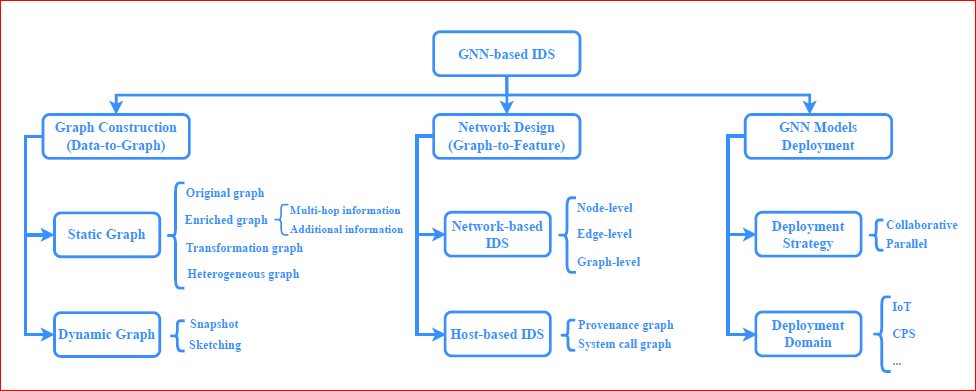
\includegraphics[width=0.8\linewidth, trim=3pt 4pt 4pt 4pt, clip]{figures/gnn1.png}
    \caption{GNN classification axes for IDS}
    \label{fig:gnn1}
\end{figure}

\textbf{GNN Methods Used in APT Detection:}
Each framework uses a distinct GNN architecture applied to provenance graphs:

\begin{table}[H]
\centering
\caption{GNN Frameworks for APT Detection}
\medskip
\scalebox{0.6}{%
\begin{tabular}{|l|l|p{7cm}|l|}
\hline
\textbf{Framework} & \textbf{GNN Used} & \textbf{Method} & \textbf{Detection Level} \\
\hline
MAGIC \cite{jia2023magic} & GAT \cite{velickovic2017gat} & Masked graph autoencoder; reconstructs masked nodes/edges via self-supervised learning & Node + graph \\
\hline
KAIROS \cite{cheng2023kairos} & TGN \cite{rossi2020tgn} & Temporal encoder-decoder; detects anomalous edges by reconstruction error over time & Graph-level \\
\hline
GCA \cite{ye2023gca} & GCN \cite{kipf2016gcn} & Graph Competitive Autoencoder with separate benign/attack decoders & Graph-level \\
\hline
DEEPRO \cite{yan2022deepro} & MAGNN \cite{fu2020magnn} & 3-metapath MAGNN on heterogeneous process graphs & Node-level \\
\hline
GHUNTER \cite{cheng2023ghunter} & GIN \cite{xu2018gin} & Subgraph matching; embeds provenance nodes & Node-level \\
\hline
THREATRACE \cite{wang2022threatrace} & GraphSAGE \cite{hamilton2017graphsage} & Inductive node-role learning on evolving provenance graphs & Node-level \\
\hline
XFedGraph-Hunter \cite{son2023xfed} & TGraphSAGE + FL \cite{ying2019gnnexplainer} & Transformer-augmented GraphSAGE with Federated Learning; uses GNNExplainer & Node-level (fed.) \\
\hline
\end{tabular}%
}
\end{table}

\textbf{Results (Table 3.5):}
Key performance metrics across PIDS and datasets (MAGIC and THREATRACE perform consistently well; GCA and GHUNTER lack transparency on ground-truth details).

\begin{table}[H]
\centering
\caption{Performance Analysis of GNN Approaches}
\medskip
\begin{tabular}{|l|l|c|c|c|c|}
\hline
\textbf{Dataset} & \textbf{PIDS} & \textbf{Precision} & \textbf{Recall} & \textbf{F1-Score} & \textbf{FPR} \\
\hline
Streamspot & MAGIC / KAIROS / THREATRACE & 1.0 & 1.0 & 1.0 & 0.0 \\
E3-Cadets & MAGIC & 0.94 & 0.997 & 0.97 & 0.22 \\
E3-Theia & MAGIC & 0.98 & 0.99 & 0.99 & 0.14 \\
E3-Theia & KAIROS & 0.82 & 1.0 & 0.90 & 0.88 \\
E5-Cadets & KAIROS & 0.44 & 1.0 & 0.60 & 3.54 \\
ATLAS & DEEPRO & 0.99 & 0.99 & 0.99 & 0.006 \\
E3-Cadets & GHunter / XFedGraph & 0.96 & 0.95--1.0 & 0.96 & --- \\
\hline
\end{tabular}
\end{table}

Figure \ref{fig:gnn2} visualizes the GAT usage in MAGIC.

\begin{figure}[H]
    \centering
    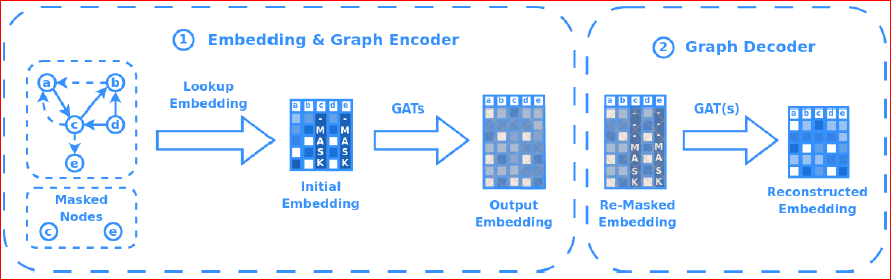
\includegraphics[width=0.8\linewidth, trim=3pt 4pt 4pt 4pt, clip]{figures/gnn2.png}
    \caption{GAT usage in MAGIC}
    \label{fig:gnn2}
\end{figure}

\subsection{Generative AI Solutions}

\subsubsection{Autoencoders (AE)}
Autoencoders are deterministic neural networks composed of an encoder that compresses input data into a compact latent representation, and a decoder that reconstructs the original input. They are trained by minimizing the reconstruction error between the input $x$ and its reconstruction $\hat{x}$:
\begin{equation}
    \mathcal{L}(\theta, \phi; x) = \| x - f_\theta(g_\phi(x)) \|^2
\end{equation}
In APT detection, autoencoders are conventionally trained exclusively on benign network traffic. During inference, inputs that deviate from the learned normal patterns yield a high reconstruction error, flagging them as potential anomalies. This unsupervised nature makes autoencoders ideal for APT detection, as labeled multi-stage attack data is often scarce.

\subsubsection{Variational Autoencoders (VAE)}
VAEs are probabilistic generative models. Unlike standard autoencoders that learn a deterministic mapping, VAEs map inputs to a probability distribution (latent space). 
\begin{equation}
    \mathcal{L}(\theta, \phi; x) = -D_{KL}(q_\phi(z|x) || p_\theta(z)) + \mathbb{E}_{q_\phi(z|x)}[\log p_\theta(x|z)]
\end{equation}
In APT detection, VAEs are trained on benign traffic. During inference, they reconstruct input data; a high reconstruction error combined with the probabilistic uncertainty metric indicates a potential malicious anomaly. \cite{ankalaki2025cyber} identifies VAEs as superior for modeling uncertainty in detection systems.

\textbf{Case Study: Multi-Stage Autoencoder Architecture \cite{neuschmied2022apt}}

\cite{neuschmied2022apt} proposed a two-stage anomaly detection architecture combining multiple autoencoder variants for APT detection.

\textbf{Architecture Used:}
The models evaluated include:
\begin{itemize}
    \item \textbf{Standard Autoencoder (AE):} Multiple dense layers trained exclusively on benign data.
    \item \textbf{Convolutional Autoencoder (AE-CNN):} Combines 1D convolutional layers with dense layers. The full architecture and data processing pipeline can be seen in Figure \ref{fig:autoen}.

\begin{figure}[H]
    \centering
    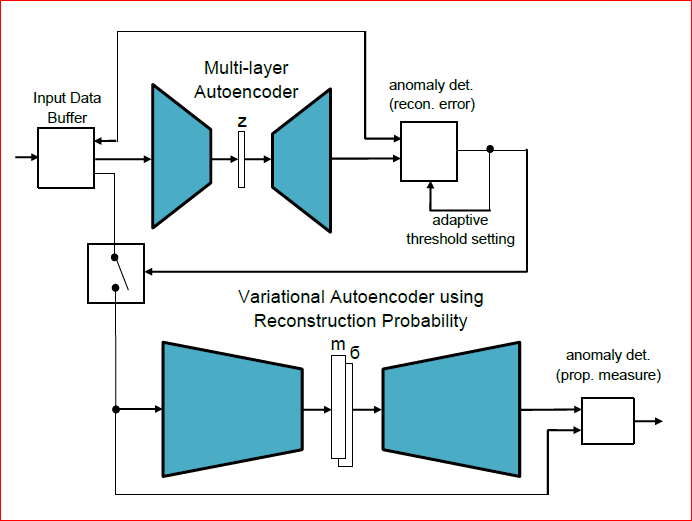
\includegraphics[width=0.6\linewidth, trim=3pt 4pt 4pt 4pt, clip]{figures/autoen.png}
    \caption{Architecture and Data Pipeline for the Autoencoder Model}
    \label{fig:autoen}
\end{figure}
    \item \textbf{Variational Autoencoder (VAE):} A sampling-based autoencoder with dense layers.
    \item \textbf{Probabilistic Variational Autoencoder (VAE-Prob):} Probability-based reconstruction with dense layers.
    \item \textbf{AE + VAE-Prob (Two-Stage):} The core novel contribution. A fast AE in stage 1 filters out clearly normal traffic, then a more precise VAE or VAE-Prob in stage 2 makes the final anomaly decision.
    \item \textbf{Baselines:} One-Class SVM (OCSVM) and AE with Custom Loss (AEC - a supervised AE).
\end{itemize}

\textbf{Methodology \& Dataset:}
The pipeline involves data pre-processing (statistical analysis, PCA) where features were reduced from 78 to 54 after removing redundant and error values. Hyperparameter optimization was done via the Talos framework optimized on AUC-ROC. 
Two publicly available datasets were combined: \textbf{CICIDS2017} provided the benign background data (5 days of enterprise traffic), while the \textbf{Contagio} dataset provided real APT malware campaigns (e.g., BIN\_9002, TrojanPage, etc.). These were merged using IP remapping, and CICFlowMeter extracted features from PCAP files. 

\textbf{Results \cite{neuschmied2022apt}:}
The multi-stage approach was evaluated on two test sets. The AE+VAE-Prob model provided a strong balance between performance and computational efficiency.

\begin{table}[H]
\centering
\caption{Results for Independent Test (18.52\% Contamination) and Zero-Day Attack Test (19.93\% Contamination) }
\resizebox{\textwidth}{!}{%
\begin{tabular}{|l|c|c|c||c|c|c|}
\hline
& \multicolumn{3}{c||}{\textbf{Independent Test Dataset}} & \multicolumn{3}{c|}{\textbf{Zero-Day Attack Test Dataset}} \\
\hline
\textbf{Method} & \textbf{Balanced Accuracy} & \textbf{F1 Score} & \textbf{Time (s)} & \textbf{Balanced Accuracy} & \textbf{F1 Score} & \textbf{Time (s)} \\
\hline
AE & 0.870 & 0.716 & 9.56 & 0.596 & 0.346 & 10.28 \\
AE-CNN & 0.797 & 0.708 & 14.17 & - & - & - \\
VAE & 0.808 & 0.670 & 243.04 & - & - & - \\
VAE-Prob & 0.847 & 0.650 & 286.31 & 0.621 & 0.394 & 250.70 \\
\textbf{AE+VAE-Prob} & \textbf{0.873} & \textbf{0.713} & \textbf{93.25} & \textbf{0.655} & \textbf{0.452} & \textbf{79.10} \\
OCSVM & 0.801 & 0.679 & 44,305.81 & 0.588 & 0.326 & 43,237.95 \\
AEC (supervised) & 0.949 & 0.913 & 4.56 & - & - & - \\
\hline
\end{tabular}%
}
\end{table}

\subsubsection{Transformers}
Transformers utilize self-attention mechanisms to weigh the importance of different parts of the input sequence, regardless of their distance in time. They are increasingly used to predict the \textit{next stage} of an attack sequence by analyzing logs, offering better parallelization and context understanding than LSTMs .

\paragraph{Case Study 2: LogShield --- Transformer-Based APT Detection via Provenance Graphs \protect\cite{anjum2023logshield}}

\cite{anjum2023logshield} proposed LogShield, a generalized APT detection framework that leverages transformer-based language models on system provenance graph-derived event traces, addressing the limitations of RNN/LSTM-based approaches in handling large-scale, long-range log sequences.

\textbf{Architecture Used:} LogShield consists of three stacked processing layers:

\begin{itemize}
    \item \textbf{Data Preprocessing Layer (Provenance Graph Builder):} Raw system log data is parsed to construct a provenance tree representing parent-child causal relationships between system events. Event traces (sequences of object-action pairs with timestamps) are generated by traversing from leaf to root nodes. All traces are padded to a uniform length (average of 31 events per trace on the DARPA OpTC dataset).
    \item \textbf{Embedding Layer:} Two custom embedding sub-layers are used jointly:
    \begin{itemize}
        \item \textit{Log Embedding:} Each event's object-action pair (e.g., FileRead, ProcessCreate) is encoded as a natural language token. A special [DTC] token marks the start and [END] marks the end of each sequence. Random token masking is applied during training following the BERT Masked Language Modeling (MLM) strategy.
        \item \textit{Temporal Embedding:} A sliding window technique divides log keys into time slots, encoding the time difference between parent and child events. This is critical for detecting APT attacks due to their characteristically slow-and-steady temporal patterns. Each time slot value is normalized by dividing by the total number of slots to keep values $\leq 1$.
    \end{itemize}
    \item \textbf{Transformer Layer (RoBERTa-based):} Multiple stacked self-attention layers learn contextual relationships among log keys. A custom Log Key Cross-Entropy Loss function trains the model to accurately predict masked log keys, enriching the separation between benign and malicious event sequences. The output is a binary classification (benign vs.\ malicious trace).
\end{itemize}

\begin{figure}[H]
    \centering
    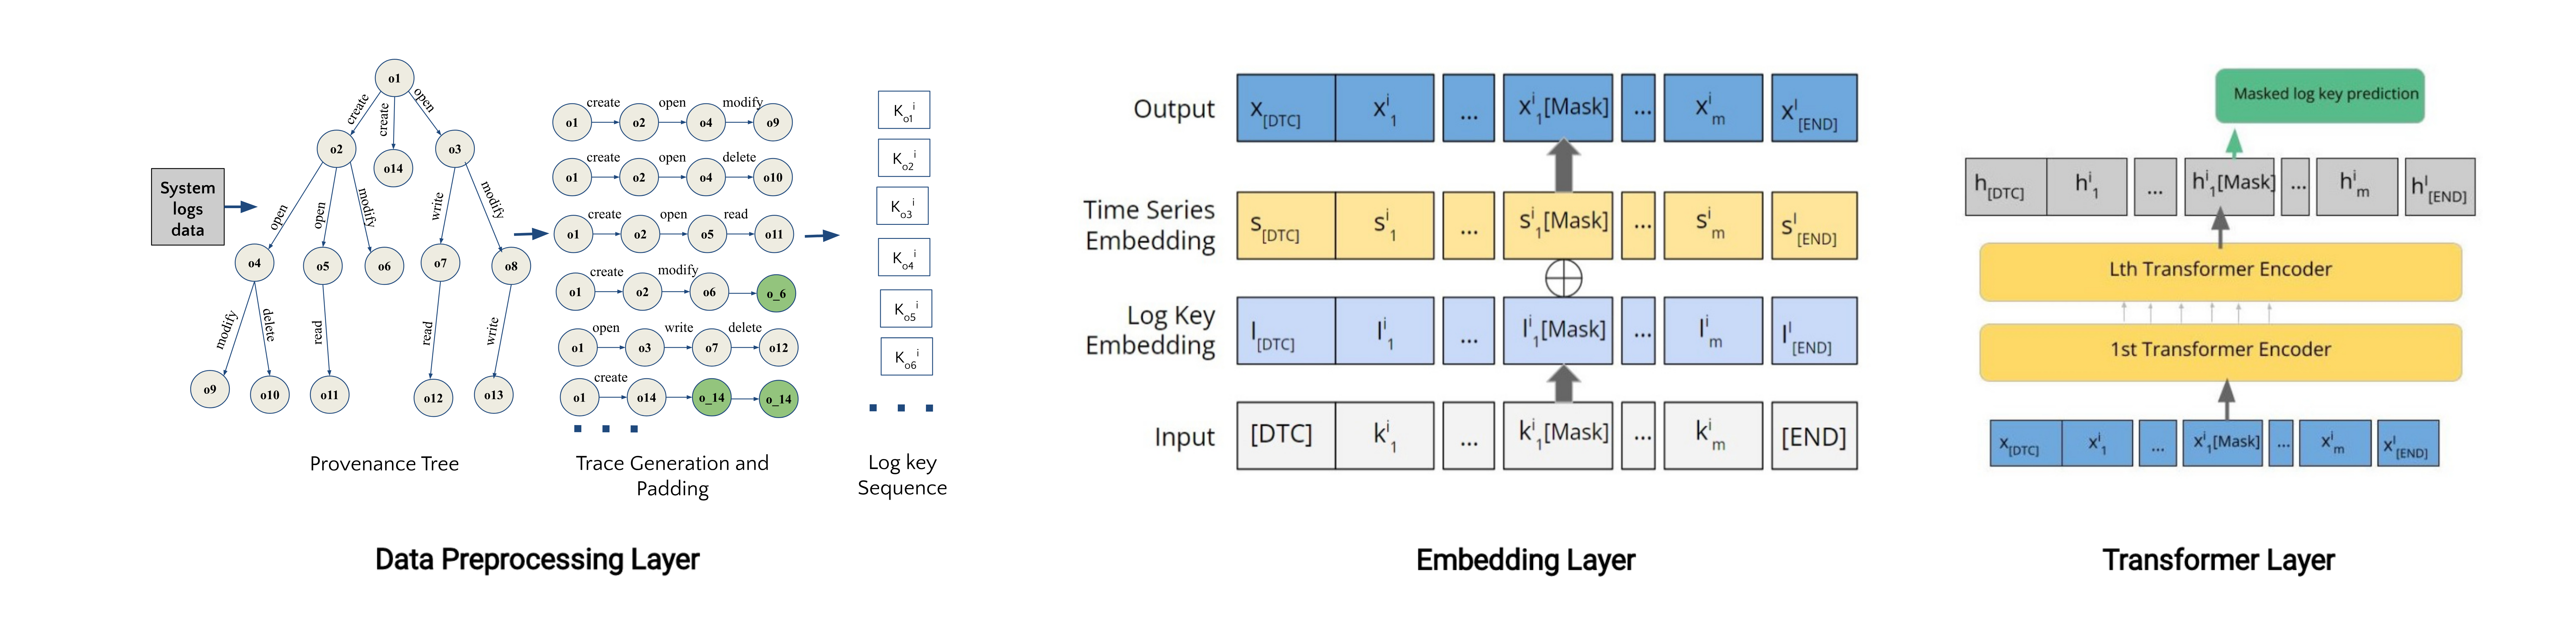
\includegraphics[width=1.1\linewidth, trim=500pt 0pt 0pt 0pt, clip]{figures/te_archi.png}
    \caption{Overview of LogShield's Architecture \protect\cite{anjum2023logshield}}
    \label{fig:te_archi}
\end{figure}

\textbf{Methodology \& Dataset:} Two publicly available DARPA datasets were used for validation:

\begin{itemize}
    \item \textbf{DARPA OpTC Dataset:} Event logs from 3 Windows hosts (SysClient0201, SysClient0321, SysClient0501), containing over 17 billion events with only 0.0016\% being malicious. A total of 103,329 benign and 20,924 malicious event traces were extracted. The provenance graph comprised 4 object types and 8 action types (32 possible object-action pairs).
    \item \textbf{DARPA TCE3 Dataset:} Data from host TA1-Cadets with 17 event types (READ, WRITE, OPEN, CONNECT, MODIFY, EXECUTE, MMAP, etc.), yielding 19,152 benign and 9,455 malicious traces. Class imbalance was handled by downsampling benign traces to an optimal count determined experimentally.
\end{itemize}

A pre-trained RoBERTa model was fine-tuned with adjusted hyperparameters (larger mini-batches, higher learning rates, removal of next-sentence pretraining objective). Training was performed on a workstation with an Intel Core i7-10750H (2.6 GHz), 16 GB RAM.

\textbf{Results \cite{anjum2023logshield}:} LogShield was evaluated against BERT, GPT-2, and LSTM baselines across both datasets. The results are summarized below:

\begin{table}[H]
\centering
\caption{Performance Comparison of LogShield with Baseline Models on DARPA Datasets}
\medskip
\resizebox{\textwidth}{!}{
\begin{tabular}{|l|c|c|c|c|c|c|c|c|}
\hline
\textbf{Model} & \textbf{OpTC Precision} & \textbf{OpTC Recall} & \textbf{OpTC Accuracy} & \textbf{OpTC F1} & \textbf{TCE3 Precision} & \textbf{TCE3 Recall} & \textbf{TCE3 Accuracy} & \textbf{TCE3 F1} \\ \hline
LogShield & 0.98 & 0.99 & 0.99 & 0.984 & 0.95 & 0.95 & 0.96 & 0.95 \\ \hline
LSTM & 0.97 & 0.97 & 0.98 & 0.96 & 0.95 & 0.94 & 0.93 & 0.944 \\ \hline
GPT-2 & 0.92 & 0.92 & 0.94 & 0.92 & 0.90 & 0.94 & 0.91 & 0.92 \\ \hline
BERT & 0.89 & 0.91 & 0.95 & 0.90 & 0.85 & 0.89 & 0.88 & 0.87 \\ \hline
\end{tabular}
}
\end{table}

LogShield consistently outperforms all baselines, particularly as training data size grows. However, it incurs higher memory consumption and longer training times compared to LSTM. LSTM remains competitive for shorter traces and memory-constrained environments, as language models may over-focus on global patterns at the expense of local sequential signals.

\subsubsection{Case Study 2: GenAI-Based Threat Intelligence Model \protect\cite{albayrak2025genai}}

\cite{albayrak2025genai} proposed a GenAI/LLM-based threat intelligence system for classifying cybersecurity threats from heterogeneous data sources. The paper emphasizes both threat classification and a comparison with traditional tools such as Splunk, Snort, and ELK Stack.

\textbf{Architecture Used:} The system is organized into three layers:

\begin{itemize}
    \item \textbf{Data collection and preprocessing layer:} Multi-source threat data are gathered, cleaned, normalized, and labeled.
    \item \textbf{Feature extraction and vectorization layer:} Text and structured data are transformed using TF-IDF, Word2Vec, and transformer-based embeddings.
    \item \textbf{Threat classification and reporting layer:} A fine-tuned GPT-3.5-based Transformer performs classification, supported by a 24-layer architecture, 8,192-token context window, and about 780 million parameters.
\end{itemize}

\textbf{Methodology \& Dataset:} The model was trained on about 2.8 million threat records from multiple sources, including MITRE ATT\&CK, VirusTotal, AlienVault OTX, CICIDS2017/2018/2019/2023, MalwareBazaar, PhishTank, CTI reports, and honeypot data. The authors also used preprocessing steps such as duplicate removal, outlier handling, translation of multilingual text, and stratified splitting into 70\% training, 15\% validation, and 15\% testing.

\begin{figure}[H]
    \centering
    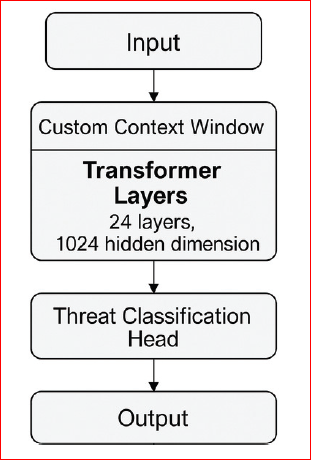
\includegraphics[width=0.3\linewidth, trim=3pt  3pt 3pt 3pt, clip]{figures/genai.PNG}
    \caption{Overview of GBTI Architecture \protect\cite{albayrak2025genai}}
    \label{fig:gbti}
\end{figure}

\textbf{Results \cite{albayrak2025genai}:} The model achieved 96.2\% accuracy, 94.5\% F1-score, 3.1\% false positive rate, and 342 ms average prediction time. For specific attacks, it reached 95.2\% accuracy on phishing, 96.8\% on DDoS, and 93.7\% on malware, while zero-day detection was lower at 82.9\%. Compared with traditional tools, it showed better overall accuracy and especially stronger zero-day detection.


\subsection{Hybrid Solutions}

\subsubsection{Case Study: GCN-Based Detection and DQN Strategic Response Model \protect\cite{shen2023sr2apt}}

\cite{shen2023sr2apt} proposed a novel two-engine host-based APT detection and response model called SR2APT, combining graph-based classification with deep reinforcement learning for proactive defense against multistage APT attacks in cyber-physical systems (CPS).

\textbf{Architecture Used:} The system consists of two independent but sequentially connected engines:



\textbf{GCN Detection Engine:} A Graph Convolutional Network that classifies provenance subgraphs extracted from host-level system logs into one of seven classes (six APT stages + benign). It uses three graph convolutional layers, each followed by a pooling layer, a dense layer, and a final output layer with softmax activation and cross-entropy loss.

\textbf{DQN Decision Engine:} A Deep Q-Network agent that receives the stream of GCN classification outputs as its environment state and outputs the optimal response action. It uses an 8-dimensional state vector \(s = (c_0, c_1, c_2, c_3, c_4, c_5, c_6, c_s)\) tracking historical class occurrence counts and the current GCN signal.

\textbf{Baselines (Detection):} Support Vector Machine (SVM), 1D Convolutional Neural Network (CNN), and Long Short-Term Memory (LSTM) network.

\textbf{Baselines (Response):} Two fixed-rate policies --- aggressive (p=1.0, always take active defense) and moderate (p=0.5, defend half the time).

\begin{figure}[H]
    \centering
    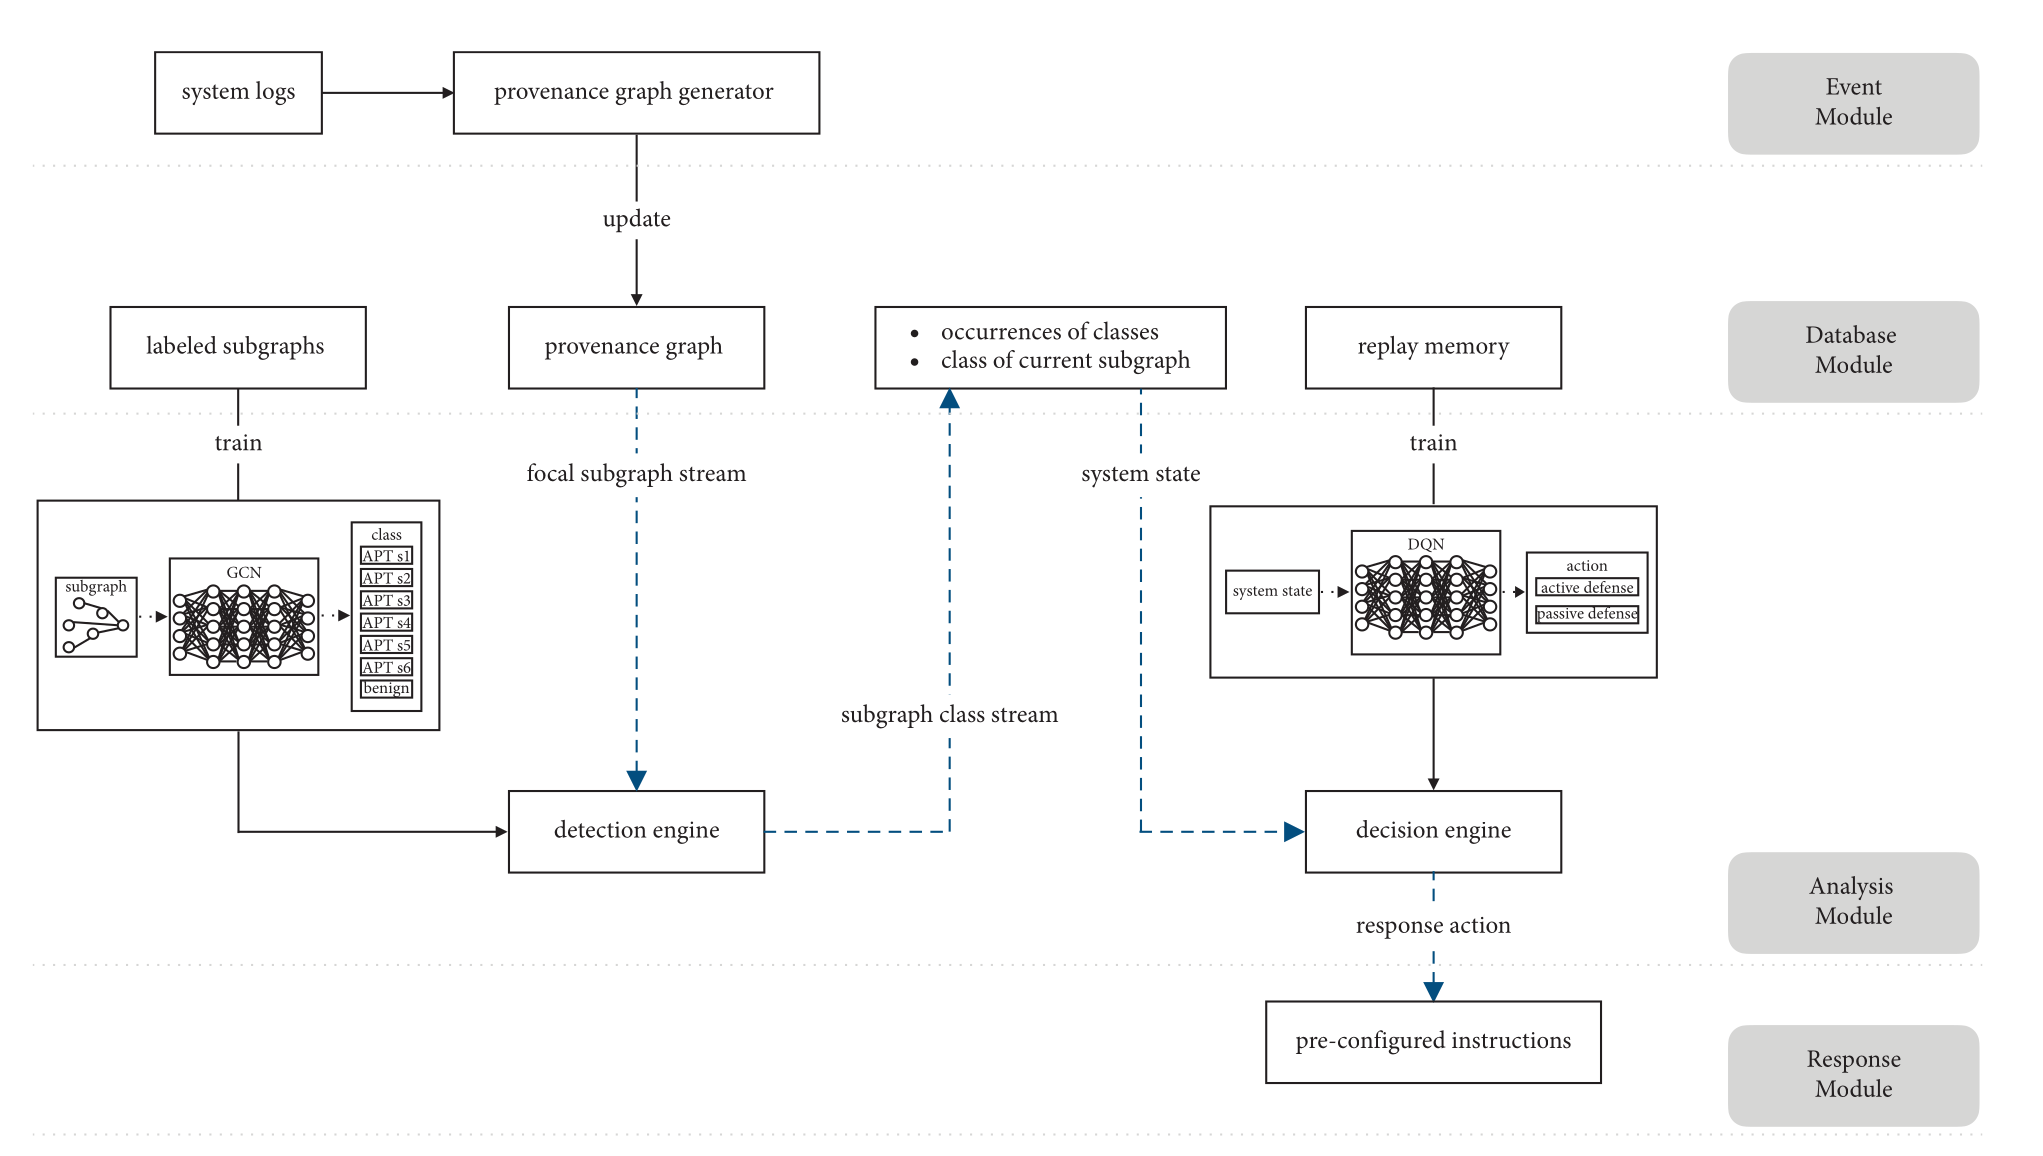
\includegraphics[width=0.9\linewidth]{figures/S2apt_architecture.png}
    \caption{Overview of SR2APT Architecture \protect\cite{anjum2023logshield}}
    \label{fig:s2rapt}
\end{figure}

\textbf{Methodology \& Dataset:} System call logs were collected on a Linux host using Sysdig (up to 57 fields per event), and GrAALF was used to parse logs, store them in a graph database, and extract labeled provenance subgraphs by traversing backwards/forwards from predefined nodes of interest (e.g., whoami $\rightarrow$ S1, su $\rightarrow$ S4). The resulting semisynthetic dataset contains 2,100 subgraphs (300 per class), split 80/10/10 for training, validation, and testing. The GCN propagation rule follows:

\begin{equation}
X^l = \sigma(\tilde{D}^{-1/2} \tilde{A} \tilde{D}^{-1/2} X^{l-1} \Theta^l)
\end{equation}
where \(\tilde{A} = A + I\) adds self-loops to the adjacency matrix. For the DQN agent, fully synthetic alert traces were generated at a ratio of AAPT:BAPT = 3:7, with parameters: damage base \(d=4\), defense cost \(c=1.5\), false alarm penalty \(p=1.5\), and active defense effectiveness \(e=0.9\).

\textbf{Results \cite{shen2023sr2apt}:} The GCN detection engine was evaluated on the semisynthetic subgraph dataset, and the DQN decision engine was evaluated over 10 iterations of 100 episodes each against synthetic alert traces.

\begin{table}[H]
    \centering
    \caption{F1-Scores of Classification Models per APT Stage \protect\cite{shen2023sr2apt}}
    \begin{tabular}{|l|c|c|c|c|c|c|c|c|}
        \hline
        Method & Benign & S1 & S2 & S3 & S4 & S5 & S6 & Overall Acc. \\
        \hline
        SVM & 1.00 & 0.52 & 0.96 & 0.80 & 0.73 & 0.89 & 0.89 & 83\% \\
        CNN & 0.98 & 0.65 & 0.95 & 0.72 & 0.77 & 0.89 & 0.90 & 84\% \\
        LSTM & 0.95 & 0.62 & 1.00 & 0.88 & 0.87 & 0.78 & 0.87 & 86\% \\
        GCN (SR2APT) & 0.91 & 0.96 & 0.98 & 0.89 & 0.90 & 0.97 & 1.00 & 94\% \\
        \hline
    \end{tabular}
\end{table}

\begin{table}[H]
    \centering
    \caption{DQN Agent Performance vs. Fixed-Rate Baselines \protect\cite{shen2023sr2apt}}
    \begin{tabular}{|l|c|c|c|}
        \hline
        Policy & Total Reward & Attacks Prevented & Mistaken Defenses on Benign \\
        \hline
        Fixed p=1.0 & $\sim-10,000$ (negative) & $\sim$Almost all & $\sim$3,000--4,000 \\
        Fixed p=0.5 & $\sim-5,000$ (negative) & Significantly fewer & $\sim$1,500--2,000 \\
        DQN (SR2APT) & $\sim+5,000$ (positive, growing) & $\sim$Almost all & $\sim$Near zero \\
        \hline
    \end{tabular}
\end{table}

\textbf{Explanation:} The GCN outperforms all baselines on 5 out of 7 classes, achieving 94\% overall accuracy. Its strongest performance is on S1 (0.96) and S6 (1.00), which are respectively the most critical stages to catch early and the most damaging to miss. Its only relative weakness is the Benign class (0.91 vs. SVM's 1.00), meaning it generates slightly more false alarms on normal activities --- precisely the problem the DQN agent was designed to handle. The DQN agent achieves the unique combination of preventing nearly all real attacks while generating almost zero disruption to benign activities, something neither fixed-rate baseline can accomplish. The agent also learns to prioritize early-stage intervention (S1--S3: $\sim$13--14 active defenses/iteration) over late-stage response (S5: $\sim$6/iteration), exploiting the sequential nature of APT kill chains. Notably, the paper does not report overall precision, recall, or FPR numerically, and includes no ablation study to validate individual component contributions.

\subsubsection{Case Study: MSL-DEEPAPT Multimodal Fusion \protect\cite{wang2025msldeepapt}}

\cite{wang2025msldeepapt} propose a multimodal deep-learning framework (MSL-DEEPAPT) for early, interpretable detection of Advanced Persistent Threats by fusing heterogeneous logs from network, endpoint, and cloud sources.

\textbf{Architecture Used:}

\begin{itemize}
    \item \textbf{Log normalization:} Ontology-based parsing and sliding time windows (default 10 minutes) produce unified event representations.
    \item \textbf{Text encoder (Windows event logs):} BiLSTM-CRF for named-entity recognition and anomaly scoring (BiLSTM hidden units = 128).
    \item \textbf{Network encoder (NetFlow):} 1D-CNN with dilated convolutions to capture long-range dependencies (kernel size = 5; dilation used).
    \item \textbf{Endpoint encoder:} Transformer encoders to model process-level behavioral sequences (8 attention heads).
    \item \textbf{Cross-modal fusion:} Attention-based alignment that constructs an entity graph (nodes: IPs/users/processes; edges: interactions) and dynamically weights modalities.
    \item \textbf{Graph aggregation \& classifier:} Graph embeddings (dim = 256) feed a multi-task prediction head that outputs binary malicious/benign and hierarchical MITRE-ATT\&CK phase labels via hierarchical softmax. Composite loss balances detection and phase classification.
\end{itemize}

\textbf{Methodology \& Dataset:}

\begin{itemize}
    \item \textbf{Preprocessing:} Ontology parsing, regex extraction, time-window alignment, SHAP used for explainability; temporal windows handle clock skew up to $\sim$30s.
    \item \textbf{Training:} Multi-task supervised training with composite loss; hyperparameters tuned (batch size 64). Baselines: Isolation Forest, LSTM autoencoder, and IBM QRadar SIEM.
    \item \textbf{Dataset:} Hybrid cloud testbed (42 VMs: Windows Server 2019, Ubuntu 20.04, Kubernetes); simulated APT campaigns via CALDERA/Metasploit produced $\sim$1.2 TB raw logs across 780 attack instances covering all 14 Enterprise MITRE tactics. Labels assigned by semi-automated mapping (STIX/TAXII) and expert verification (Cohen's kappa = 0.89).
\end{itemize}

\begin{figure}[H]
    \centering
    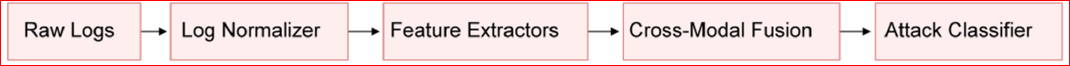
\includegraphics[width=0.9\linewidth,trim= 3pt 3pt 3pt 3pt,clip]{figures/msl.png}
    \caption{MSL-DEEPAPT System Architecture}
    \label{fig:msl}
\end{figure}

\textbf{Results \cite{wang2025msldeepapt}:}

\begin{itemize}
    \item \textbf{Global test detection accuracy:} 92.3\% (MSL-DEEPAPT) vs lower single-source baselines.
    \item \textbf{Lateral movement recall:} 89.7\%.
    \item \textbf{False positives:} 41.2\% reduction vs commercial SIEM baseline.
    \item \textbf{Detection latency (average by phase):} Initial access 2.3 $\pm$0.4 min, Lateral movement 8.7 $\pm$1.2 min.
    \item \textbf{Throughput:} up to $\sim$78,000 log entries/sec in distributed tests; processing latency (95th percentile) under $\sim$1.2s in testbed.
\end{itemize}

\begin{table}[H]
    \centering
    \caption{Selected MSL-DEEPAPT results (excerpt) \protect\cite{wang2025msldeepapt}}
    \medskip
    \begin{tabular}{|l|l|}
        \hline
        \textbf{Metric} & \textbf{Value} \\
        \hline
        Detection accuracy & 92.3\% \\
        Lateral movement recall & 89.7\% \\
        False-positive reduction vs SIEM & 41.2\% \\
        Avg lateral movement latency & 8.7 min \\
        Throughput (distributed) & 78,000 EPS (95th pctl latency $\sim$1.2s) \\
        \hline
    \end{tabular}
\end{table}

\subsubsection{Case Study: StageFinder \& DeepStage --- Provenance-Graph APT Detection and Defense \protect\cite{phan2026learning, phan2026deepstage}}

\cite{phan2026learning, phan2026deepstage} developed a two-paper research series addressing both the detection and the autonomous defense sides of Advanced Persistent Threat (APT) campaigns. The first paper, StageFinder \cite{phan2026learning}, introduces a temporal-graph learning framework for APT kill-chain stage estimation. The second, DeepStage \cite{phan2026deepstage}, extends this work by integrating StageFinder's stage inference component into a deep reinforcement learning (DRL) agent capable of selecting adaptive defense actions in real time. Both frameworks are grounded in fused host and network provenance data, and together they form a complete detection-to-response pipeline.

\textbf{Architecture Used:}

The full system is structured as a five-component pipeline, with StageFinder covering the first three components and DeepStage adding the last two:

\begin{figure}[H]
    \centering
    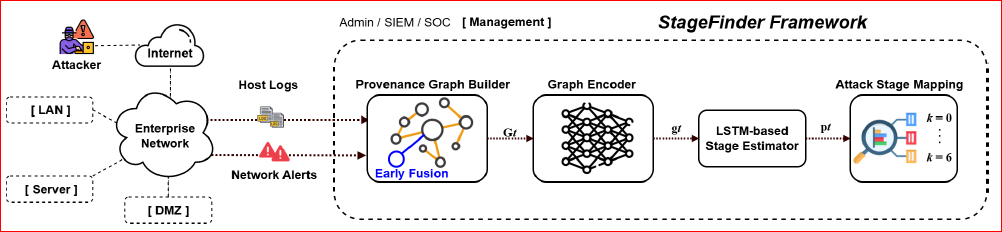
\includegraphics[width=\linewidth]{figures/stagefinder.png}
    \caption{Architecture and workflow of StageFinder \protect\cite{phan2026learning}}
    \label{fig:stagefinder}
\end{figure}

\begin{itemize}
    \item \textbf{Provenance Graph Builder:} Raw host logs (Sysmon, Auditd) and network alerts (Zeek, Snort) are parsed and correlated into fused provenance graphs $G_t = (V_t, E_t)$, where nodes represent system entities (processes, files, sockets, IPs, users, and alert events) and directed edges encode causal or temporal dependencies (spawn, read, write, connect, triggered\_by). An early fusion mechanism links network alert nodes directly to the responsible host processes during graph construction, preserving causal completeness across both modalities.
    \item \textbf{GNN Encoder:} A multi-layer Graph Neural Network performs message passing over each fused graph snapshot and produces a fixed-length embedding $g_t \in \mathbb{R}^{d_g}$ via attention-based readout, compactly representing both intra-host and inter-host structural dependencies.
    \item \textbf{LSTM-Based Stage Estimator (StageFinder):} A two-layer LSTM (hidden size 128, dropout 0.3) processes the sequence of graph embeddings $g_1, \ldots, g_t$ and outputs a probability distribution over seven classes --- one benign class plus six MITRE ATT\&CK stages (Reconnaissance, Initial Compromise, Privilege Escalation, Lateral Movement, Command \& Control, Exfiltration) --- via a softmax classifier.
\end{itemize}

\begin{figure}[H]
    \centering
    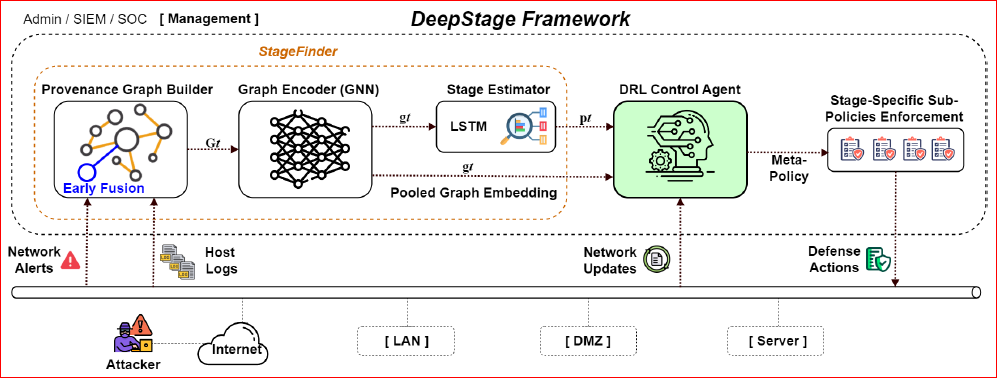
\includegraphics[width=\linewidth]{figures/deepstage.png}
    \caption{Architecture and workflow of DeepStage \protect\cite{phan2026deepstage}}
    \label{fig:deepstage}
\end{figure}

\begin{itemize}
    \item \textbf{Hierarchical PPO Agent (DeepStage):} The graph embedding $g_t$ and the stage belief vector $p_t$ are combined into a unified state observation fed to a hierarchical Proximal Policy Optimization (PPO) agent. A meta-policy selects among four structured defense categories, and each corresponding sub-policy executes one of 29 concrete, automatable actions.
    \item \textbf{Action Hierarchy:} The four meta-policy categories are: Monitoring (e.g., increase log verbosity, deploy deep packet inspection), Access Control (e.g., revoke sessions, enforce MFA), Containment (e.g., isolate hosts, block malicious IPs, kill processes), and Remediation (e.g., patch vulnerabilities, rollback to snapshots, restore from backup).
\end{itemize}

\textbf{Methodology \& Dataset:}

StageFinder was trained in two sequential phases. First, self-supervised pretraining is performed on the large unlabeled DARPA OpTC dataset ($\sim$8.7 billion host events + 0.53 billion Zeek flow logs), using next-step prediction and a temporal contrastive loss to learn generic host-network temporal dynamics. Second, supervised fine-tuning is applied on the labeled DARPA Transparent Computing (TC) dataset, which contains multi-week red/blue-team engagements (200--600 million records across Linux, FreeBSD, and Windows hosts) with ground-truth MITRE ATT\&CK stage annotations. Logs are segmented into 300-second windows, and all experiments are run in PyTorch 2.1 with DGL on an NVIDIA RTX 3060 GPU.

DeepStage models the defense problem as a Partially Observable Markov Decision Process (POMDP), since the true security state is only partially observable through logs and alerts. Instead of replay datasets, it uses a controlled enterprise testbed of six Ubuntu 20.04 VMs and one Kali Linux attacker VM. Attack scenarios are generated programmatically using MITRE Caldera, producing 10 base ATT\&CK-aligned multi-stage playbooks with randomized variants, each annotated with ground-truth stage labels. Stage-conditioned reward weights $\alpha_k$ and $\beta_k$ are tuned per APT phase --- favoring low-cost monitoring in early stages and escalating to aggressive containment or remediation as the attack progresses toward Exfiltration.

\textbf{Results \cite{phan2026learning, phan2026deepstage}:}

StageFinder was evaluated on DARPA TC Engagement 5 against two baselines: Cyberian (LSTM on host events only) and NetGuardian (stage-specific ensemble classifiers):

\begin{table}[H]
    \centering
    \caption{Performance Comparison of StageFinder vs. Baselines \protect\cite{phan2026learning}}
    \begin{tabular}{|l|c|c|c|}
        \hline
        \textbf{Metric} & \textbf{Cyberian} & \textbf{NetGuardian} & \textbf{StageFinder} \\
        \hline
        Precision & 0.89 $\pm$ 0.02 & 0.92 $\pm$ 0.02 & 0.96 $\pm$ 0.01 \\
        Recall & 0.90 $\pm$ 0.03 & 0.91 $\pm$ 0.02 & 0.96 $\pm$ 0.01 \\
        F1-Score & 0.90 $\pm$ 0.02 & 0.92 $\pm$ 0.02 & 0.96 $\pm$ 0.01 \\
        Accuracy & 0.90 $\pm$ 0.03 & 0.92 $\pm$ 0.02 & 0.96 $\pm$ 0.01 \\
        AUPR & 0.91 $\pm$ 0.02 & 0.94 $\pm$ 0.02 & 0.97 $\pm$ 0.01 \\
        TFR ($\downarrow$) & 0.182 & 0.160 & 0.125 \\
        \hline
    \end{tabular}
\end{table}

StageFinder improved the macro F1-score from 0.90 / 0.92 to 0.96, and reduced prediction volatility (Temporal Flip Rate) by 31\%, reflecting more stable stage transitions over time. Per-stage gains were consistent across all phases, with C2 reaching F1 = 0.97 and Exfiltration reaching 0.95.

DeepStage was benchmarked against Risk-Aware DRL (static attack-graph baseline) and DeepStage-Unaware (same framework without stage conditioning):

\begin{table}[H]
    \centering
    \caption{Mitigation Success Rate and F1 Score of DeepStage vs. Baselines \protect\cite{phan2026deepstage}}
    \begin{tabular}{|l|c|c|}
        \hline
        \textbf{Method} & \textbf{Avg F1} & \textbf{Mitigation Success Rate} \\
        \hline
        Risk-Aware DRL & 0.728 & 68.5\% \\
        DeepStage-Unaware & 0.797 & 76.7\% \\
        DeepStage & 0.887 & 84.7\% \\
        \hline
    \end{tabular}
\end{table}

DeepStage improved mitigation success by +16.2\% over the Risk-Aware DRL baseline and by +8\% over its stage-unaware variant. It also converged 1.7$\times$ faster ($\sim$900 training episodes vs. $\sim$1,600--1,800 for the baselines), achieved a normalized episodic reward of 0.91 at convergence, and reached a defense responsiveness of 0.97 by the fourth timestep ($\sim$20 minutes of emulated time). At mid-range operational cost, DeepStage attained a security gain of 0.65, outperforming DeepStage-Unaware (0.54) and Risk-Aware DRL (0.43) by 23\% and 51\% respectively.

\section{Comparative Analysis}

\begin{table}[H]
    \centering
    \caption{Comparative Analysis of Related Works}
    \resizebox{\textwidth}{!}{%
    \begin{tabular}{|l|l|l|c|c|c|c|c|c|c|c|c|l|}
        \hline
        \textbf{Solution / Model} & \textbf{Category} & \textbf{Dataset} & \textbf{Acc.} & \textbf{Precision} & \textbf{Recall} & \textbf{F1} & \textbf{Temporal} & \textbf{Unsupervised} & \textbf{APT-Specific} & \textbf{Early Det.} & \textbf{Model Fusion} & \textbf{Key Limitation} \\
        \hline
        Takey et al. (2021) --- RF & Traditional ML & Custom PE (Windows) & 98.18\% & --- & --- & --- & $\times$ & $\times$ & $\checkmark$ & $\times$ & $\times$ & Static PE only, no sequence \\
        Saad \& Yildiz (2023) --- DQN & Traditional ML + RL & NSL-KDD & 93.12\% & 96.83\% & 95.90\% & 0.964 & $\times$ & $\times$ & $\times$ & $\times$ & $\times$ & Outdated dataset, no APT stages \\
        Naive Bayes & Traditional ML & CICIDS2017 & --- & --- & low & 0.040 & $\times$ & $\times$ & $\times$ & $\times$ & $\times$ & Independence assumption fails \\
        CNN2D (Sharmila Devi et al., 2026) & Deep Learning & CICAPT-IIoT & 99.78\% & 99.7\% & 99.8\% & 0.998 & $\times$ & $\times$ & $\checkmark$ & $\times$ & $\times$ & Spatial only, no temporal modeling \\
        AISL (Yue et al., 2024) --- LSTM & Deep Learning & Structured audit logs & 99.98\% & 93.05\% & 98.12\% & 0.954 & $\checkmark$ & $\times$ & $\checkmark$ & $\times$ & $\times$ & Brittle on noisy logs \\
        LogShield (Anjum et al., 2023) --- Transformer & Deep Learning & DARPA OpTC / TCE3 & 99\% & 0.98 & 0.99 & 0.984 & $\checkmark$ & $\times$ & $\checkmark$ & $\times$ & $\times$ & High memory, no semantic embeddings \\
        MAGIC (Jia, 2023) --- GAT & Deep Learning & E3-Cadet / Theia & --- & 0.94 & 0.997 & 0.97 & $\checkmark$ & $\checkmark$ & $\checkmark$ & $\times$ & $\times$ & Graph construction overhead \\
        KAIROS (Cheng et al., 2023) --- TGN & Deep Learning & E3-Theia / E5 & --- & 0.82 & 1.00 & 0.90 & $\checkmark$ & $\checkmark$ & $\checkmark$ & $\times$ & $\times$ & High FPR on large graphs \\
        THREATRACE --- GraphSAGE & Deep Learning & Streamspot / E3 & --- & 1.00 & 1.00 & 1.00 & $\checkmark$ & $\checkmark$ & $\checkmark$ & $\times$ & $\times$ & Limited real-world evaluation \\
        Neuschmied et al. (2022) --- AE+VAE & Generative AI & CICIDS2017 + APT & --- & --- & --- & 0.713 & $\times$ & $\checkmark$ & $\checkmark$ & $\times$ & $\checkmark$ & Low zero-day accuracy (0.655) \\
        Albayrak et al. (2025) --- GPT-3.5 & Generative AI & Multi-source & 96.2\% & --- & --- & 0.945 & $\times$ & $\times$ & $\checkmark$ & $\times$ & $\times$ & No sequence modeling, costly \\
        SR2APT (Shen et al., 2023) --- GCN+DQN & Hybrid & Semisynthetic Linux & 94\% & --- & --- & 0.94 & $\checkmark$ & $\times$ & $\checkmark$ & $\sim$ & $\checkmark$ & Semisynthetic only, no real APT data \\
        MSL-DEEPAPT (Wang et al., 2025) & Hybrid & Hybrid Cloud testbed & 92.3\% & --- & 89.7\% & --- & $\checkmark$ & $\times$ & $\checkmark$ & $\sim$ & $\checkmark$ & No GenAI augmentation \\
        StageFinder+DeepStage (Phan et al., 2026) & Hybrid & DARPA TC / OpTC & 96\% & 0.96 & 0.96 & 0.96 & $\checkmark$ & $\times$ & $\checkmark$ & $\times$ & $\checkmark$ & No synthetic data, offline only \\
        \hline
    \end{tabular}%
    }
\end{table}

Temporal ($\checkmark$) indicates the approach captures time-ordered event sequences. Unsupervised ($\checkmark$) means the approach does not require labeled attack data. APT-Specific ($\checkmark$) means evaluation was conducted on a dataset with APT or CKC-relevant characteristics. Early Detection ($\checkmark$) indicates the framework explicitly intercepts the attack before its final objectives; ($\sim$) indicates partial early detection --- the system is stage-aware but does not explicitly optimize for pre-objective interception. Model Fusion ($\checkmark$) indicates the solution combines outputs from multiple models rather than relying on a single classifier. 

The table reveals a clear progression across the three generations of solutions. Traditional ML methods --- Random Forest, SVM, Naive Bayes --- achieve competitive accuracy on well-defined benchmark datasets but treat every security event as an independent observation. They carry no notion of attack sequencing, making them structurally incapable of detecting the slow, multi-stage progression that defines APT campaigns. Their strong numbers on datasets like CICIDS2017 are therefore misleading in the APT context: high accuracy on isolated events does not translate to early kill-chain interception.

Deep learning models represent a significant step forward, particularly graph-based approaches. MAGIC, KAIROS, and THREATRACE demonstrate that modeling the structural and temporal relationships between system entities --- rather than individual events --- dramatically improves detection on APT-relevant provenance datasets. THREATRACE achieves perfect scores on Streamspot, while MAGIC reaches F1 = 0.97 on the more challenging E3-Cadets benchmark. However, even these strong performers share two critical blind spots: none incorporate early detection as an explicit objective, and none fuse outputs from multiple heterogeneous models. Each solution commits to a single architecture, leaving complementary signals from other model families unexploited.

The transformer-based LogShield confirms that sequential log modeling benefits from attention mechanisms, achieving F1 = 0.984 on DARPA OpTC. Yet it relies on generic tokenization of log events and does not leverage domain-specific security language models, leaving the semantic richness of log content --- process names, command arguments, alert descriptions --- largely untapped.

Generative AI solutions occupy a distinct niche. The AE+VAE-Prob architecture of Neuschmied et al. demonstrates that unsupervised anomaly detection on benign-only training data is viable for APT scenarios where labeled attack samples are scarce, though its zero-day F1 of 0.452 reveals clear generalization limits. Albayrak et al. show that large language models can classify threat types effectively, but apply GenAI as a discriminator rather than as a data generator --- missing its most impactful potential use in the APT domain: generating novel, structurally valid attack sequences to expand training coverage.

The hybrid solutions --- SR2APT, MSL-DEEPAPT, and StageFinder/DeepStage --- represent the current state of the art and are the only approaches that combine kill-chain awareness with multi-model architectures and early detection intent. StageFinder/DeepStage in particular achieves the best overall balance across all dimensions, with F1 = 0.96, explicit stage estimation across all six CKC phases, and adaptive defense through a PPO agent. Nevertheless, even this strongest baseline operates without synthetic data augmentation, without semantic log embeddings, and without live operational deployment --- evaluated exclusively on offline DARPA datasets that, while rich, do not cover the full diversity of real-world APT TTPs.

Taken together, the comparative analysis points to a convergence of unresolved challenges: the need to model attack sequences across the full kill chain, to augment training data with generative techniques that produce novel APT patterns, to exploit the semantic content of logs through domain-specific embeddings, and to fuse the complementary strengths of multiple detection architectures under a learned arbitration mechanism. These are precisely the four pillars of the framework proposed in Chapter 3.

\subsection{Limitations of Existing Solutions}

The comparative analysis of reviewed solutions reveals five recurring structural limitations that collectively define the boundaries of current APT detection research.

\textbf{Limited multi-stage modeling.} Most approaches treat security events as independent observations, with no mechanism to correlate them into coherent attack narratives. Traditional ML models operate entirely at the event level, and even deep learning solutions struggle to maintain state across the extended dwell times characteristic of real APT campaigns. Only a few hybrid frameworks (SR2APT, StageFinder) explicitly model kill-chain progression.

\textbf{Absence of generative augmentation.} APT datasets are inherently scarce and biased toward known threat groups, causing models to overfit to observed TTPs and generalize poorly to novel adversarial sequences. No reviewed solution addresses this through generative synthesis of structurally valid APT data, leaving zero-day detection performance critically limited.

\textbf{Underexploitation of semantic log content.} The majority of solutions discard rich textual information embedded in logs — process names, command-line arguments, and alert descriptions — relying instead on flow-level statistics. Domain-specific embeddings such as SecBERT, capable of capturing semantic relationships between TTPs and log entries, are absent from every reviewed pipeline.

\textbf{Single-model architectures.} Nearly all reviewed solutions commit to a single architecture, forgoing the complementary strengths of autoencoders (anomaly detection), transformers (sequential dependencies), and graph neural networks (structural relationships). No work learns to dynamically fuse these signals — a role naturally suited to a reinforcement learning agent.

\textbf{Research-to-deployment and dataset gaps.} Every reviewed solution is evaluated on offline datasets under laboratory conditions, with no integration into live SIEM systems or operational SOC workflows. Furthermore, widely used benchmarks such as NSL-KDD and CICIDS2017 lack kill-chain annotations, making them ill-suited for stage-aware APT evaluation and rendering cross-study comparisons unreliable.

These limitations directly motivate the design of the proposed framework, which targets each dimension through an integrated combination of sequential deep learning, generative augmentation, semantic embeddings, multi-model fusion, and operational SIEM deployment.